\documentclass[11pt]{article}
\usepackage[utf8]{inputenc}
\usepackage[T1]{fontenc}
\usepackage{amsmath,amssymb}
\usepackage[version=4]{mhchem}
\usepackage{graphicx}
\usepackage{booktabs}
\usepackage{siunitx}
\usepackage[margin=1in]{geometry}
\usepackage[hidelinks]{hyperref}
\usepackage{xr-hyper}
\externaldocument[][nocite]{main}[main.pdf]
\usepackage[numbers,sort&compress]{natbib}
\usepackage{caption}
\usepackage{tocloft}
\captionsetup{font=small,labelfont=bf}
\setlength{\cftsecnumwidth}{3.2em}
\setlength{\cftsubsecnumwidth}{4.0em}
\renewcommand{\thefigure}{S\arabic{figure}}
\renewcommand{\thetable}{S\arabic{table}}
\renewcommand{\theequation}{S\arabic{equation}}
\renewcommand{\thesection}{S\arabic{section}}
\newcommand{\epss}{\varepsilon_{\mathrm{s}}}
\newcommand{\iapp}{i_{\mathrm{app}}}
\newcommand{\csat}{c_{\mathrm{sat}}}
\newcommand{\epsl}{\varepsilon}
\newcommand{\Deff}{D_{\mathrm{eff}}}
\newcommand{\thetaeff}{\theta_{\mathrm{eff}}}
\newcommand{\thetacal}{\theta_{\mathrm{cal}}}
\newcommand{\thetaisland}{\theta_{\mathrm{island}}}
\newcommand{\epscalstar}{\varepsilon_{\mathrm{s,cal,traj}}^{*}}
\newcommand{\epsislandhalf}{\varepsilon_{\mathrm{s,island},1/2}}
\newcommand{\epsfilmperc}{\varepsilon_{\mathrm{s,film\text{-}perc}}^{*}}
\newcommand{\mAhcm}{\si{mAh.cm^{-2}}}
\newcommand{\ci}{c_{\mathrm{I^-}}}
\newcommand{\cf}{c_{\mathrm{I_2}}^{\,\mathrm{f}}}
\DeclareSIUnit{\Molar}{M}

\title{\bfseries Supplementary Information for \textit{A zinc--iodine flow-battery positive-electrode model
coupling solid-iodine deposition and accessibility loss}\\[3pt]
\normalsize\mdseries Reduced iodine-state framework, implementation map, molecular priors and mesoscale closures}
\author{}
\date{}

\begin{document}
\maketitle
\tableofcontents
\bigskip

\section{Governing equations of the continuum positive-electrode scaffold}

\paragraph{Roadmap and registered branch.} This section specifies the continuum scaffold for the ZIFB
positive electrode under full-cell boundary conditions. We first distinguish solved primary fields,
algebraic closures, calibrated effective relations and prescribed inputs (Table~\ref{tab:implmap}), and then
give the species, charge, kinetic and solid-phase balances, geometry, flow, areal source basis, reservoir,
boundary and initial conditions. The registered production identity is:
\begin{quote}\small
branch \texttt{PB-R526-J40-Q120-DSET5-v1}; source SHA-256
\texttt{4813B306...B8806B9B} (full hash in the matched-branch manifest); study \texttt{stdR522};
solution \texttt{sol5}; dataset \texttt{dset5}.
\end{quote}
A read-only identity probe explicitly
confirmed \texttt{dset5}$\rightarrow$\texttt{sol5}. The SI symbols $\varepsilon$ and
$\varepsilon_{l,\mathrm{eff}}=\varepsilon-\epss$ are the main text's initial felt porosity
$\varepsilon_0$ and running pore-liquid fraction $\varepsilon_l$. Throughout, $S_{\mathrm{base}}$ is the
within-electrolyte production stress. Supporting-electrolyte composition is treated separately and does not
alter the native stress-field identity.

\begin{table}[tb]\centering
\caption{Implementation-to-theory map for the registered continuum positive-electrode scaffold. Each object
is classified by how it is produced in the native run, verified from the exported time series (baseline,
$\iapp=\SI{400}{A.m^{-2}}$, $q:0\to\SI{120}{mAh.cm^{-2}}$). ``Solved'' $=$ primary state advanced by a
balance/ODE; ``consequence'' $=$ evaluated pointwise on a solved field; ``closure'' $=$ algebraic function
of a solved field; ``calibrated closure'' $=$ an algebraic relation whose effective magnitude is constrained
by voltage; ``prescribed'' $=$ imposed boundary input.}
\label{tab:implmap}\small
\begin{tabular}{@{}p{2.3cm}p{3.2cm}p{1.9cm}p{4.9cm}@{}}
\toprule
object & exported source & status & data evidence / wording\\
\midrule
$c_R=\ce{I-}$ & \texttt{cI\_m\_surf\_avg} & algebraic consequence & $1688\!\to\!704~\si{mol.m^{-3}}$ ($-58\%$); registered inventory $\max(c_{R,\mathrm{floor}},c_{R,0}-3c_O)$\\
$c_O$ (\ce{I3-}, \ce{I2Br-}, \ce{I2(aq)}) & native transported state (not separately exported in the registered
figure table) & solved & transported oxidized-iodine inventory advanced by the species balance\\
surface-effective total/free \ce{I2} and $S$ & surface total/free exports; \texttt{S\_direct} & algebraic consequence & combines the solved inventory,
boundary-layer generation term and $\beta$; the $q{=}0$ surface total is ${\approx}104~\si{mol.m^{-3}}$
while stored inventory is ${\approx}0$; $S:0.19\!\to\!1.76$\\
$\beta$ (buffer) & \texttt{beta\_surf\_avg} & algebraic consequence & identity $\beta=1+K_{\mathrm I}c_R+K_{\mathrm{Br}}c_{\mathrm{Br}}$ on reconstructed $c_R$; $1263\!\to\!554$\\
$\epss$ (\ce{I2(s)}) & \texttt{eps\_s\_avg} & solved (native deposited species) & $\partial_t\epss=V_m a_sj_{\mathrm{dep}}/(2F)$; $0\!\to\!3.2\times10^{-3}$\\
$\varepsilon_{\mathrm{s,aux}},N_{\mathrm{I_2}}$ & \texttt{eps\_s\_i2}, \texttt{N\_i2} & solved auxiliary ODE states & smooth phase-transfer tracker ends at $1.08\times10^{-6}$; $N_{\mathrm{I_2}}$ enters only the calibrated accessibility relation\\
$\thetacal,A_{\mathrm{bare}}$ & \texttt{theta\_avg} & calibrated closure & evaluated on native $\epss$ and dynamic $N_{\mathrm{I_2}}$; $A_{\mathrm{bare}}=(1-\thetacal)K_{\mathrm{rel}}^{1/2}$\\
$\varepsilon_{l,\mathrm{eff}},K,D,\kappa_l$ & \texttt{eps\_l\_eff\_avg}, \texttt{K\_perm\_rel\_avg} & closure & algebraic in $\epss$ (Kozeny--Carman / Bruggeman); $K_{\mathrm{rel}}:1.00\!\to\!0.96$\\
$\mathbf{u},p$ (flow) & \texttt{u\_native\_mag\_avg}, \texttt{p\_native\_avg} & solved (two-way FPF) & feedback negligible: solved $u$ varies $<\!0.1\%$ as $\epss$ grows $3$ decades; identical saturation marker in a frozen-velocity control\\
model terminal voltage & \texttt{voltage\_V} & solved (galvanostatic) & $1.40\!\to\!1.73~\si{V}$ within the voltage-calibrated accessibility parameterization\\
\bottomrule
\end{tabular}
\end{table}


The native positive-electrode model under full-cell boundary conditions is a tertiary-current-distribution
problem coupled to Darcy flow, a native deposited-species state and two parallel auxiliary ODE states. With
$O$ the transported lumped oxidized-iodine pool (\ce{I3-}, \ce{I2Br-}, \ce{I2(aq)}), the registered species
and stoichiometric-inventory relations are
\begin{align}
c_R&=\max(c_{R,\mathrm{floor}},c_{R,0}-3c_O),\\
\varepsilon\,\partial_t c_O+\nabla\!\cdot(\mathbf{u}c_O-D_{O,\mathrm{eff}}\nabla c_O)
&=R_{\mathrm b}-R_{\mathrm{dep}}+(r_{\mathrm d}-r_{\mathrm p})/V_m,
\end{align}
where $R_{\mathrm b}=a_{\mathrm b}j_{\mathrm b}/(2F)$ and
$R_{\mathrm{dep}}=a_sj_{\mathrm{dep}}/(2F)$. Thus $c_O$ is the transported species field; $c_R$ is a
depleting algebraic inventory and must not be described as a second solved species. Charge is conserved through
$i_v=a_{\mathrm b}j_{\mathrm b}+a_sj_{\mathrm{dep}}$,
$\nabla\!\cdot\mathbf{i}_s=-i_v$, $\nabla\!\cdot\mathbf{i}_l=+i_v$,
$\mathbf{i}_s=-\sigma_{s,\mathrm{eff}}\nabla\phi_s$ and
$\mathbf{i}_l=-\kappa_{l,\mathrm{eff}}\nabla\phi_l$.

The bare-carbon path uses constant-exchange-current Butler--Volmer kinetics,
\begin{equation}
\begin{aligned}
j_{\mathrm b}&=i_0\!\left[e^{\alpha_aF\eta/RT}-e^{-\alpha_cF\eta/RT}\right],\qquad
\eta=\phi_s-\phi_l-E_{\mathrm{eq}},\\
E_{\mathrm{eq}}&=E^{0\prime}+\gamma_a\frac{RT}{2F}\ln\!\left[
\frac{\max(\cf,c_{\mathrm f})}{c_{\mathrm{ref}}/\beta}\right]+\eta_{\mathrm{tank}},\qquad
a_{\mathrm b}=a_s(1-\theta)K_{\mathrm{rel}}^{1/2}.
\end{aligned}
\end{equation}
The registered values are $i_0=5\times10^{4}~\si{A.m^{-2}}$, $\alpha_a=\alpha_c=1$,
$E^{0\prime}=\SI{0.548}{V}$, $c_{\mathrm{ref}}=\SI{120}{mol.m^{-3}}$,
$c_{\mathrm f}=\SI{0.02}{mol.m^{-3}}$ and $\gamma_a=1$. All generic concentration reaction orders are
zero. Because $\cf=c_O/\beta$, this implemented expression reduces away from the floor to a total-pool
Nernst-like term. It is an empirical potential closure, not a thermodynamically complete activity expression.
The charge-only window ends before $\eta_{\mathrm{tank}}$ activates.

The second active positive-electrode feature is a native-solid anodic Tafel path,
\begin{equation}
\begin{aligned}
j_{\mathrm{dep}}&=i_{0,\mathrm{dep}}10^{\eta/A_a},\qquad
i_{0,\mathrm{dep}}=i_{0,\mathrm{dep}}^{\mathrm{base}}\max(S_{\mathrm{local}}-1,0),\\
\partial_t\epss&=V_mR_{\mathrm{dep}},\qquad
\partial_t\varepsilon_{\mathrm{s,aux}}=r_{\mathrm p}-r_{\mathrm d},\qquad
\partial_tN_{\mathrm{I_2}}=\kappa_N(N_{\mathrm{target}}-N_{\mathrm{I_2}}),
\end{aligned}
\end{equation}
with $i_{0,\mathrm{dep}}^{\mathrm{base}}=\SI{0.05}{A.m^{-2}}$ and $A_a=\SI{118}{mV}$. The native
deposited-species fraction $\epss$ is the state used by all transport and accessibility closures. The
parallel smooth tracker $\varepsilon_{\mathrm{s,aux}}$ enters the $c_O$ balance through
$(r_{\mathrm d}-r_{\mathrm p})/V_m$ but does not drive $N_{\mathrm{I_2}}$ and does not define the reported
retained-solid inventory. The $N_{\mathrm{I_2}}$ state evolves independently through its target-relaxation
equation and enters the calibrated accessibility relation. The algebraic feedback closures are
\begin{equation}
\varepsilon_{l,\mathrm{eff}}=\varepsilon-\epss,\quad
K=\Big(\tfrac{\varepsilon_{l,\mathrm{eff}}}{\varepsilon}\Big)^3\Big(\tfrac{1-\varepsilon}{1-\varepsilon_{l,\mathrm{eff}}}\Big)^2,\quad
\{D,\kappa_l\}\!\propto\!\Big(\tfrac{\varepsilon_{l,\mathrm{eff}}}{\varepsilon}\Big)^{3/2},\quad
\thetacal=1-\exp\!\left[-6N_{\mathrm{I_2}}^{1/3}\varepsilon_{\mathrm{s,reg}}^{2/3}\right].
\label{eq:closures-ref}
\end{equation}
At the canonical endpoint, $\epss=3.21926\times10^{-3}$ while
$\varepsilon_{\mathrm{s,aux}}=1.08328\times10^{-6}$; the ratio is $2972$. The native-solid path carries
$0.552\%$ of integrated charge and $27.99\%$ of endpoint positive current. Local $S>1$ activates that path
before the electrode-average $S=1$ marker, so $Q_{\mathrm s}$ is a registered mean surface-effective
saturation marker, not the first local supersaturation or first solid.
Here $N_{\mathrm{I_2}}$ is a dynamic dimensionless production-model state, not a fixed physical areal
density. The physical isolated-island relation is defined separately in Sec.~\ref{sec:meso}. The reported
COMSOL terminal voltage is a solved galvanostatic scaffold output rather than a fitted polynomial; comparison
with the selected experimental voltage trace instead uses a calibrated reduced observation layer.

\subsection{Geometry, domains, and the compression rule}\label{sec:geom}
The native problem is posed in two dimensions---the through-plane coordinate $x\in[0,L]$ spanning the
compressed positive electrode of thickness $L$, bounded at $x=0$ by the current collector and at $x=L$ by the
ion-selective membrane, and the flow-wise coordinate $y$ along the channel---with a well-mixed tank reservoir
(Sec.~\ref{sec:tankbc}) feeding and draining the pore space; the reduced criterion reads the through-plane
profile.
The deposited-solid fraction $\epss(x,t)$ is referred to the total electrode volume, consistent with the
closure $\varepsilon_{l,\mathrm{eff}}=\varepsilon-\epss$ above (verified end-of-charge:
$\epss+\varepsilon_{l,\mathrm{eff}}=0.85$ to twelve figures). Mechanical compression is imposed at fixed
fiber inventory, so squeezing the felt lowers $L$ and $\varepsilon$ together,
\begin{equation}
(1-\varepsilon)\,L=\SI{0.30}{mm}=\mathrm{const},
\label{eq:compress}
\end{equation}
and the compression series is a one-parameter family in $L$ (equivalently $\varepsilon$) at constant solid
loading.

\subsection{Electrolyte flow and the permeability closure}\label{sec:flow}
Convection in the pore space is a Darcy field layered on the solved electrode state,
\begin{equation}
\mathbf{u}=-\frac{\kappa_0\,K(\epss)}{\mu}\,\nabla p,\qquad \nabla\!\cdot\mathbf{u}=0,
\label{eq:darcy}
\end{equation}
with $\mathbf{u}$ the superficial velocity, $p$ the pore pressure, $\mu$ the viscosity, $\kappa_0$ the
deposit-free permeability, and $K(\epss)$ the relative-permeability closure of Eq.~\eqref{eq:closures-ref}
(Kozeny--Carman form, refined by the pore-network model of Sec.~\ref{sec:meso}). The advective flux
$\mathbf{u}\,c_i$ enters the species balances above. Explicit species electromigration is omitted from this
reduced transport operator; ionic current is instead represented through the charge-conservation equation
with a prescribed effective liquid conductivity. The formal potential $E^{0\prime}$ represents reaction
thermodynamics and is not a proxy for a migration flux. The velocity is solved \emph{together with} the electrochemistry: the native porous-media-flow interface
solves $\mathbf{u},p$ and feeds the solved $\mathbf{u}$ back into the species convection (full two-way
coupling), with the permeability multiplier $K/K_0$ a smooth, monotone, single-valued closure of the solved
solid inventory (unity at $\epss=0$, decreasing thereafter). In practice this feedback is negligible: across
a full charge the solved $\mathbf{u}$ is constant to $<\!0.1\%$ even as $\epss$ grows by three orders of
magnitude, and a control solve with the velocity frozen gives the \emph{identical} saturation marker. The reason
is that $K/K_0$ stays $\approx\!1$ until the accessibility threshold is already crossed ($K/K_0=0.998$ at
$\theta_{\mathrm{eff}}{=}\tfrac12$), so within the analyzed pre-failure window the pressure rises by only a few percent.
Far past failure the feedback is no longer benign: as the pore network fully clogs ($K/K_0\!\to\!0$, reaching
$\approx\!0.25$ in the most diffusion-limited case at $\theta_{\mathrm{eff}}\!\to\!1$) the Darcy pressure diverges
super-linearly, rising $\sim\!10^{3}\times$ toward $\sim\!\SI{8}{bar}$ in the frozen-throughput limit ---
the regime in which constant-flow pumping mechanically ruptures tubing and seals in practice. This
extrapolation is reported only as a post-failure hydraulic consequence, not as a fitted or validated
operating threshold. That fully-destabilised hydraulic runaway is a distinct, deep-post-failure mode downstream of the
accessibility-collapse failure analyzed here and lies outside the present continuum scope; we therefore use
the in-window solution to quantify the (mild) hydraulic consequence of \ce{I2}(s) accumulation, and make no
claim of a flow-coupled voltage validation.

\subsection{Areal basis of the two faradaic paths and the through-thickness reduction}\label{sec:areabasis}
With $a_s$ the pristine specific area, the bare-carbon path has
$a_{\mathrm b}=a_s(1-\theta_{\mathrm{eff}})K_{\mathrm{rel}}^{1/2}$, whereas the native-solid path uses
$a_s$. Their volumetric rates are
\begin{equation}
R_{\mathrm b}=\frac{a_{\mathrm b}j_{\mathrm b}}{2F},\qquad
R_{\mathrm{dep}}=\frac{a_sj_{\mathrm{dep}}}{2F},\qquad
i_v=2F(R_{\mathrm b}+R_{\mathrm{dep}}).
\label{eq:rgen}
\end{equation}
The bare path produces the transported oxidized pool and the deposited-species path consumes that pool while
forming native solid. Galvanostatic charge balance therefore requires
\begin{equation}
\int_0^L\!\left(R_{\mathrm b}+R_{\mathrm{dep}}\right)\mathrm{d}x
=\frac{1}{2F}\int_0^L\!i_v\,\mathrm{d}x
=\frac{\iapp}{2F}.
\label{eq:Jgen}
\end{equation}
The reduced generation group $\Pi_{\mathrm{gen}}$ uses $\iapp/2F$ as the total charge-equivalent supply and
omits an explicit $a_sL$ factor. In the canonical charge, the native-solid path accounts for only $0.552\%$
of integrated charge, so this is a close areal approximation to soluble-pool generation, but it is not an exact
identity at each instant. Accessibility loss reshapes both the spatial current distribution and the late
bare-versus-solid current partition.

\subsection{Reservoir coupling, boundary, and initial conditions}\label{sec:tankbc}
The transported oxidized-iodine pool is coupled to a well-mixed tank of volume $V_{\mathrm{tank}}$ at
concentration $c_O^{\mathrm{tank}}(t)$,
\begin{equation}
V_{\mathrm{tank}}\,\frac{\mathrm{d}c_O^{\mathrm{tank}}}{\mathrm{d}t}
=\dot V\bigl(c_O^{\mathrm{out}}-c_O^{\mathrm{tank}}\bigr),
\label{eq:tank}
\end{equation}
with $\dot V$ the volumetric flow rate and $c_O^{\mathrm{out}}$ the electrode outlet concentration. The
boundary conditions are
\begin{align}
\text{inlet:}&\quad c_O=c_O^{\mathrm{tank}},\quad \mathbf{u}\!\cdot\!\hat{\mathbf n}=u_{\mathrm{in}};
\label{eq:bcin}\\
\text{outlet:}&\quad -D_{O,\mathrm{eff}}\nabla c_O\!\cdot\!\hat{\mathbf n}=0,\quad p=p_{\mathrm{out}};
\label{eq:bcout}\\
\text{collector }(x{=}0):&\quad \mathbf{i}_s\!\cdot\!\hat{\mathbf n}=\iapp,\quad
\mathbf{i}_l\!\cdot\!\hat{\mathbf n}=0,\quad \nabla c_O\!\cdot\!\hat{\mathbf n}=0;
\label{eq:bccc}\\
\text{membrane }(x{=}L):&\quad \mathbf{i}_s\!\cdot\!\hat{\mathbf n}=0,\quad
\mathbf{i}_l\!\cdot\!\hat{\mathbf n}=\iapp,\quad \nabla c_O\!\cdot\!\hat{\mathbf n}=0,
\label{eq:bcmem}
\end{align}
with $\hat{\mathbf n}$ the outward normal: the iodine species are blocked at the membrane (only the
charge-balancing counter-ion crosses, carried by $\iapp$), electronic current is collected at $x=0$, and
ionic current closes the circuit at $x=L$. The native deposited \ce{I2}(s) is a purely local state with no
spatial flux and is advanced by the solid-path faradaic rate, $\partial_t\epss=V_mR_{\mathrm{dep}}$.
The initial state is start-of-charge equilibrium: uniform $c_O(x,0)=c_{O,0}$, algebraic
$c_R(x,0)=\max(c_{R,\mathrm{floor}},c_{R,0}-3c_{O,0})$, and zero native deposited solid
$\epss(x,0)=0$ (hence $\theta_{\mathrm{eff}}=0$, $a_{\mathrm b}=a_s$, $K=1$), with the rest potential
consistent with the prescribed reference state. In the solved baseline the reconstructed surface iodide
$c_R$ depletes monotonically (\SI{1688}{mol.m^{-3}}$\to$\SI{704}{mol.m^{-3}}, $-58\%$) as the transported
oxidized pool grows and \ce{I2}(s) accumulates. Thus $c_R$ and the buffer $\beta$ are solved-state
\emph{consequences}, not independent primary fields or prescribed time series. Every $\beta$- and
$S_{\mathrm{base}}$-based statement is evaluated on that registered algebraic inventory.

\section{Molecular priors}
The registered electronic-energy and diffusivity priors are summarized in
Tables~\ref{tab:dftenergies} and \ref{tab:mddiffusivities}; their corresponding electronic-structure panels
are shown in Figs.~\ref{fig:dft4} and \ref{fig:dft2i2}.
\begin{table}[h]\centering
\caption{Periodic DFT (D3+PBE) \ce{I2} adsorption and coalescence energies on graphitic slabs. Used as
trapping/coalescence \emph{tendencies} (nucleation placement bias), never as kinetic constants.}
\label{tab:dftenergies}
\begin{tabular}{lcc}
\toprule
site & $E_{\mathrm{ads}}$ (eV) & note\\
\midrule
basal pristine & $-0.40$ & baseline\\
carbonyl \ce{C=O} & $-0.85$ & strong O trap\\
hydroxyl \ce{C-OH} & $-1.00$ & strongest accepted trap\\
single vacancy & $-0.32$ & weaker than basal\\
\midrule
2\ce{I2} coalescence at \ce{C-OH} & $-0.69$ & coalescence favored\\
\bottomrule
\end{tabular}
\end{table}

\begin{table}[h]\centering
\caption{Molecular-dynamics carrier diffusivities in $1\,\si{M}\,\ce{ZnI2}+4\,\si{M}\,\ce{NH4Br}$
($\times10^{-9}~\si{m^2.s^{-1}}$). Each entry is the arithmetic mean of five compositionally distinct
SOC-box estimates, not a mean over replicate trajectories. This is a bounded force-field prior; only the
order and scale are used.}
\label{tab:mddiffusivities}
\begin{tabular}{lcc}
\toprule
species & $q{=}0.8$ ECC & $q{=}1.0$\\
\midrule
\ce{H2O} & 1.99 & 1.33\\
\ce{I-} & 1.22 & 0.71\\
\ce{I2} & 1.07 & 0.59\\
\ce{I3-} & 0.75 & 0.53\\
\ce{I2Br-} & 0.72 & 0.52\\
\bottomrule
\end{tabular}
\end{table}

\begin{figure}[h]\centering
\includegraphics[width=0.95\textwidth]{figures/SIFig_DFT_4panel.pdf}
\caption{Periodic CP2K single-\ce{I2} DFT. (a) Adsorption energy per \ce{I2} across basal,
hydroxyl, carbonyl and vacancy sites; (b) optimized adsorption geometries; (c) charge-density-difference
$\Delta\rho$ (accumulation blue, depletion orange) at \ce{C-OH} and \ce{C=O}; (d) \ce{I2}-projected
density of states near the Fermi level. Within this finite-cell computational setup, the maps are consistent
with stronger relative retention at the oxygenated sites and are used only as a bounded placement prior.
\emph{Convergence caveat:} these GPW
calculations use a plane-wave density cutoff of \SI{150}{Ry} (\texttt{REL\_CUTOFF} \SI{30}{Ry}) with MOLOPT
basis sets, which is adequate to rank site \emph{preferences} but not to converge absolute binding energies;
accordingly the adsorption energies are read only as a relative site-ordering (placement bias), never as
quantitative binding constants, and none enters the continuum model as a kinetic parameter.}
\label{fig:dft4}
\end{figure}

\begin{figure}[h]\centering
\includegraphics[width=0.95\textwidth]{figures/SIFig_DFT_2I2_mechanism.pdf}
\caption{Periodic CP2K 2\ce{I2} coalescence (the single-\ce{I2} adsorption baseline is in
Fig.~\ref{fig:dft4}). (a) Electronic-energy difference for a compact 2\ce{I2} configuration at \ce{C-OH}
(\SI{-0.69}{eV} relative to the registered separated reference; the \ce{C=O} result is D3-only);
(b) charge-density-difference $\Delta\rho$ for that configuration (I--I $=3.03$~\AA); (c) a possible local
association motif. These finite-cell electronic-energy diagnostics do not establish a solution free energy,
equilibrium constant, trapping event or nucleation pathway; they provide only a bounded placement prior,
with production constants unchanged.}
\label{fig:dft2i2}
\end{figure}

\section{Mesoscale closures}\label{sec:meso}
The physical single-fibre and pore-network models bound two different consequences of retained iodine; they
do not identify the magnitude of the production accessibility relation. The fitted dense isolated-island
relation is
\begin{equation}
\thetaisland(\epss)=1-\exp\!\left(-35.4\,\varepsilon_{\mathrm{s,reg}}^{0.6222}\right),
\qquad
\epsislandhalf=1.7973\times10^{-3},
\label{eq:thetaisland}
\end{equation}
where $\epsislandhalf$ is defined by $\thetaisland=\tfrac12$. Direct interpolation of the dense discrete
single-fibre output gives approximately $1.91\times10^{-3}$. A separate geometric calculation gives the
connected-film/percolation marker $\epsfilmperc=2.2324\times10^{-3}$. This marker is not a
half-accessibility definition. The production trajectory has a third quantity,
$\epscalstar=1.1898\times10^{-4}$, defined as the true-mesh control's averaged solid fraction when
$\langle\thetacal\rangle=\tfrac12$ in the fresh matched control. It is a trajectory readout of the calibrated
closure, not a material threshold. These three symbols are not interchanged anywhere in this SI.

At the true-mesh production endpoint ($\langle\epss\rangle\simeq3.15\times10^{-3}$), the tested pore-network laws
retain approximately $98$--$99\%$ of their smooth relative permeability. This result excludes only a smooth
mean-field permeability collapse over the modeled load; it does not exclude discrete local pore-throat,
shell or connected-deposit blockage.

\paragraph{Matched closure-sensitivity solve.}
The two comparison cases used independent copies of the registered source model with identical SHA-256
hashes. Both cases
used COMSOL~6.3, study \texttt{stdR522}, live solution \texttt{sol5}, mesh \texttt{mesh1} and the inherited
1081-point time grid. The control changed no expression. The physical-dense case changed only
\texttt{cov\_theta\_surf} and \texttt{theta\_eff\_R520} to Eq.~\eqref{eq:thetaisland}. Parameter inventories
were byte-identical, and each post-solve dataset was explicitly mapped to its own live \texttt{sol5}. The
fresh canonical-mesh control passed every predeclared reproduction gate against the registered R526/R525
trajectory; the
maximum absolute voltage-trace difference was \SI{0.285}{mV}, and the direct and reconstructed saturation
stresses agreed to machine precision in both cases. A tighter-tolerance pair and a second pair on a
7776-element mesh were then solved at $\mathrm{rtol}=3\times10^{-4}$. Both predeclared convergence gates
passed; relative to the same-tolerance 1944-element pair, the true-mesh endpoint voltage difference changed
by only \SI{0.094}{mV}.
The canonical registered production figures retain $Q_{\mathrm s}=83.0202$ and
$Q_{\mathrm f,cal}=99.5901~\si{mAh.cm^{-2}}$. The true-mesh control shifts these values by only
$-0.1299$ and $-0.1264~\si{mAh.cm^{-2}}$, respectively. The true-mesh pair is therefore used for the
closure comparison and convergence claim, whereas the frozen canonical branch remains the traceable source
of the registered production-state figures.

\begin{table}[h]\centering\small
\caption{Convergence-qualified true-mesh control and physical dense-island coupled solve. Endpoint values are at
$Q=\SI{120}{mAh.cm^{-2}}$. The physical-minus-control voltage difference is
$-\SI{288.156}{mV}$. This is a causal model-closure sensitivity under fixed continuum settings, not a
measurement or morphology identification.}
\label{tab:matchedclosures}
\begin{tabular}{lcc}
\toprule
quantity & production control & physical dense-island \\
\midrule
$Q_{\mathrm s}$ (\si{mAh.cm^{-2}}) & $82.8903$ & $82.8924$ \\
$Q(\langle\theta\rangle=0.5)$ (\si{mAh.cm^{-2}}) & $99.4637$ & not reached \\
$V_{\mathrm{end}}$ (V) & $1.728364$ & $1.440208$ \\
$\langle\epss\rangle_{\mathrm{end}}$ & $3.15236\times10^{-3}$ & $6.58584\times10^{-4}$ \\
$\langle\theta\rangle_{\mathrm{end}}$ & $0.989982$ & $0.309081$ \\
$K_{\mathrm{rel,end}}$ & $0.957035$ & $0.988976$ \\
\bottomrule
\end{tabular}
\end{table}

\begin{table}[tbp]\centering\small
\caption{Protocol and provenance of the molecular transport prior. The continuum calculation uses
$T=\SI{293.15}{K}$; the separate MD prior was generated at \SI{298.15}{K}.}
\label{tab:mdprotocol}
\begin{tabular}{@{}p{0.20\textwidth}p{0.24\textwidth}p{0.46\textwidth}@{}}
\toprule
item & frozen implementation & evidential boundary \\
\midrule
software and cases & GROMACS 2026.0-conda\_forge; five target SOC boxes at each of $q=0.8$ and $q=1.0$ &
one long trajectory per SOC/charge case; the ten cases are not replicate samples of one condition \\
trajectory protocol & \SI{0.1}{ns} NVT, \SI{0.5}{ns} NPT, \SI{20}{ns} NVT production; \SI{2}{fs} step;
\SI{5}{ps} saved-frame interval & \SI{298.15}{K}; V-rescale thermostat, C-rescale barostat during NPT,
PME electrostatics and \SI{1.0}{nm} real-space cutoffs \\
diffusion estimator & molecular-centre-of-mass Einstein MSD; full-trajectory lag fit
\SIrange{2.51}{8.49}{ns} & the displayed block statistic is SD$/\sqrt{4}$ from four contiguous
\SI{5}{ns} segments of the same trajectory; it is a within-trajectory stability diagnostic, not an
independent-replica SEM \\
base models & SPC/E water; Joung--Cheatham-style \ce{I^-}/\ce{Br^-}; SPC/E-compatible 12--6 \ce{Zn^2+};
compact tetrahedral \ce{NH4^+}; neutral two-site \ce{I2} & the \ce{Zn^2+}, \ce{NH4^+} and \ce{I2} models
are project approximations; no 12--6--4 \ce{Zn^2+} term or present-electrolyte force-field validation is claimed \\
polyhalides & completed GFN2-xTB 6.7.1/ALPB-water charge priors
\citep{Bannwarth2019GFN2xTB}; manual linear bonded terms and halogen-analogue Lennard--Jones terms &
absolute \ce{I3^-}/\ce{I2Br^-} diffusivities are high-uncertainty; the completed logs/charge files, rather than
the stale generated summary marked \texttt{xtb\_not\_run}, are the authoritative artifacts \\
viscosity & 18 planned Green--Kubo replica rows & all 18 lack \texttt{visc\_rep.edr}; they are not results and
support no uncertainty estimate \\
\bottomrule
\end{tabular}
\end{table}

The $q=0.8$ branch scales the ionic charges, including the xTB polyhalide charge priors, by 0.8; the formal-charge
$q=1.0$ branch brackets this force-field choice. The finite boxes retain at least one neutral \ce{I2} molecule
for mobility diagnostics even when the equilibrium free fraction would be below one molecule, and the carrier
mix is prescribed rather than reactively equilibrated. These calculations therefore support a
force-field-limited ordering of carrier mobilities, not phase equilibrium, viscosity, an absolute
concentrated-electrolyte transport coefficient or a transferable NH4Br law. The representative supporting
electrolyte remains context for the ZIFB positive-electrode model, not the modeled object of interest.

A one-way dense-island shadow evaluated on the true-mesh \emph{control} $\epss(Q)$ trajectory crosses
$\thetaisland=\tfrac12$ at $Q=\SI{118.6927}{mAh.cm^{-2}}$ and ends at $0.625898$. In the coupled physical
solve, accessibility feedback suppresses solid accumulation and the half-accessibility point is not reached;
its endpoint is $0.309081$. The one-way shadow and coupled solve are therefore different objects. The matched
$-\SI{288.156}{mV}$ difference establishes closure sensitivity, but voltage alone cannot identify whether the
real deposit is an island, a connected film, a pore-spanning structure or another blocking morphology.

\section{Voltage: accessibility--coefficient degeneracy and internal overpotential}
The absolute charge voltage does not uniquely determine deposit morphology. In the reduced observation layer,
the accessibility coefficient and a Tafel-like coefficient trade off over a broad range
(Fig.~\ref{fig:degeneracy}). The internal decomposition in Fig.~\ref{fig:eta} is therefore a conditional
description of the calibrated model, not an independent separation of physical mechanisms. The matched result
in Table~\ref{tab:matchedclosures} quantifies the response to one closure-expression change while preserving
the same continuum settings; it does not resolve the inverse morphology problem.
The smooth-permeability substitution and its small in-window voltage response are shown in
Fig.~\ref{fig:kperm}.

\begin{figure}[h]\centering
\includegraphics[width=0.92\textwidth]{figures/Fig_R538_voltage_reanchor.pdf}
\caption{\textbf{Accessibility--coefficient degeneracy in the calibrated observation layer.} Left: the selected
full-cell charge trace has a modest pre-failure rise. Right: similar voltage contributions are obtained over a
wide effective-accessibility range by trading the accessibility and Tafel-like coefficients. The voltage alone
neither establishes nor excludes an island, connected-film, pore-spanning or other blocking morphology.}
\label{fig:degeneracy}
\end{figure}

\begin{figure}[h]\centering
\includegraphics[width=0.92\textwidth]{figures/Fig_R537_eta_internal.pdf}
\caption{Conditional internal-overpotential decomposition of the calibrated continuum model across the
modeled thickness cases. Within this parameterization the electronic/contact contribution is larger than the
ionic ohmic contribution; the panel is not an experimental mechanism decomposition.}
\label{fig:eta}
\end{figure}

\begin{figure}[h]\centering
\includegraphics[width=0.9\textwidth]{figures/Fig_R537_kperm_injection.pdf}
\caption{\textbf{Bulk permeability loss is small within the smooth network closure.} Replacing the
mean-field Kozeny--Carman permeability with the physically derived pore-network closure $K(\varepsilon_s)$
and re-solving the continuum model shifts the cell voltage by only $\sim\!\SI{1.3}{mV}$; the relative
permeability stays near unity throughout (Kozeny--Carman endpoint $0.96$, pore-network endpoint $0.98$).
This rules out a smooth, mean-field permeability penalty as the dominant late-voltage driver within the
calibrated model, but does not exclude discrete or local pore-throat blockage.}
\label{fig:kperm}
\end{figure}

\section{Experimental configuration and data provenance}\label{sec:expconfig}
The reported aqueous experimental electrolytes contain \ce{ZnI2} and \ce{NH4Br}; NH4Br is the
representative supporting electrolyte, not the redox-active subject of this paper. Two cell formats are kept
strictly separate. Galvanostatic capacity, composition, compression and rate datasets are \SI{4}{cm^2} full
cells with a positive iodine felt, zinc negative electrode and Nafion~212 separator. Cyclic-voltammetry,
chronoamperometry and impedance tests use a separate \SI{1}{cm^2} three-electrode configuration with an
Ag/AgCl reference and are identified explicitly where used. No full-cell capacity is described as a
three-electrode measurement.
The retained acquisition records do not contain an independently logged or controlled cell temperature; the
experiments are therefore reported as laboratory-ambient measurements. The continuum temperature
(\SI{293.15}{K}) and MD temperature (\SI{298.15}{K}) are model settings and are not assigned retrospectively
to the experimental files.

\paragraph{Operator-confirmed NH4Br metadata correction.}
Legacy acquisition filenames and condition fields containing ``NH4Cl'' or ``NH4CL'' are metadata-entry
errors. The experimenter confirmed on 2026-07-11 that every affected experiment used NH4Br. Raw files,
filenames and SHA-256 hashes remain byte-for-byte unchanged; normalization occurs only in the analysis layer
under correction ID \texttt{EXP-META-001}. The deposited
\texttt{R581\_NH4BR\_METADATA\_CORRECTION} directory contains a 114-path manifest and a 39-unique-hash
manifest, each retaining the raw and canonical labels. The correction does not change protocol eligibility
and does not reinstate excluded, duplicated or incomplete runs.

\section{Full-cell voltage-derivative sensitivity}\label{sec:g4audit}
The voltage-derivative analysis was rebuilt directly from the full-resolution strict-pristine raw file
(SHA-256 \texttt{D276F111323AA0E6\allowbreak D9271DED881B9E6C\allowbreak 5437712931F85A34\allowbreak 30FDB5D326B6CC98}). All four
eligible repeated charge cycles at $40\pm2~\si{mA.cm^{-2}}$ and $120\pm1~\si{mAh.cm^{-2}}$ were retained;
no best cycle was selected. The primary estimator was a cubic Savitzky--Golay derivative with a
$10.25~\si{mAh.cm^{-2}}$ physical window, with $5.25$ and $15.25~\si{mAh.cm^{-2}}$ prespecified
sensitivity windows. These cycles are sequential repeats from one physical cell ($n_{\mathrm{cell}}=1$),
not independent replicates; Table~\ref{tab:g4audit} lists the resulting primary-window landmarks.

\begin{table}[tbp]\centering\small
\caption{Primary-window full-cell $\mathrm{d}V/\mathrm{d}Q$ landmarks for all eligible cycles. The
cycle- and window-dependent landmarks are different observables from the modeled saturation and calibrated
accessibility states; they do not validate their ordering.}
\label{tab:g4audit}
\begin{tabular}{ccc}
\toprule
pair & rise onset (\si{mAh.cm^{-2}}) & derivative maximum (\si{mAh.cm^{-2}})\\
\midrule
20 & 52.00 & 95.00\\
21 & 50.75 & 92.00\\
22 & 51.75 & 106.75\\
23 & 89.25 & 114.00\\
\bottomrule
\end{tabular}
\end{table}

Across the three prespecified windows, 11 of 12 rise onsets occurred before the modeled
$Q_{\mathrm s}=\SI{83.0}{mAh.cm^{-2}}$, while derivative maxima spanned
$92.0$--$115.25~\si{mAh.cm^{-2}}$ and fell on both sides of
$Q_{\mathrm f,cal}=\SI{99.6}{mAh.cm^{-2}}$. The former 62/94~\si{mAh.cm^{-2}} consistency statement is
therefore withdrawn. The existing full-cell traces do not provide a stable validation of the model ordering;
the derivative signature remains a prospective electrode-resolved test.
(Supplementary Fig.~\ref{fig:experimental-evidence}d.)

\section{Experimental compression series}\label{sec:compression}
The thickness evidence was rebuilt from all protocol-eligible full-cell cycles: 110 paired cycles were
reconstructed and 108 retained under prespecified protocol/artifact rules. Each thickness is one physical
cell ($n_{\mathrm{cell}}=1$). The 1.5, 2.5 and 3.0 mm cells are from the March 2025 explicit-thickness
campaign; the nominal 2.0 mm point is a December 2024 cross-acquisition-batch pristine cell whose thickness is
implicit in the project standard and is treated as a proxy. The CE-qualified brackets are reported in
Table~\ref{tab:compression}.

\begin{table}[h]\centering\small
\caption{Descriptive, CE-qualified capacity brackets at the primary within-cell median CE threshold of
85\%. ``Last pass'' and ``first fail'' are commanded charge-capacity levels and define an observed protocol
bracket, not a confidence interval. Delivered capacity and CE are medians at the last passing level. The
2.0 mm row is a cross-batch proxy.}
\label{tab:compression}
\begin{tabular}{lcccccc}
\toprule
$L$ & role & $n_{\mathrm{cell}}$ & last pass & first fail & delivered & CE (\%)\\
(mm) & & & \multicolumn{3}{c}{(\si{mAh.cm^{-2}})} & \\
\midrule
1.5 & explicit & 1 & 60 & 80 & 57.26 & 95.44\\
2.0 & proxy & 1 & 100 & 120 & 95.27 & 95.27\\
2.5 & explicit & 1 & 100 & 120 & 85.96 & 85.96\\
3.0 & explicit & 1 & 140 & 160 & 135.51 & 96.79\\
\bottomrule
\end{tabular}
\end{table}

The explicit March series has increasing last-pass capacity at 1.5, 2.5 and 3.0 mm under the 80, 85 and
90\% CE definitions, but inclusion of the cross-batch 2.0 mm proxy does not define a universal monotonic
scaling law. The first failing 1.5 mm level contains only one target-attained cycle before file termination.
Common-capacity voltage profiles use all eligible cycles and report within-cell ranges. Their voltage metric is
the energy-weighted mean charge--discharge gap, not a mid-capacity gap. These observations are descriptive and
protocol-bounded; they do not validate a quantitative pore-volume law or equate delivered discharge capacity
with the modeled $Q_{\mathrm f,cal}$. Because shuttle and other inefficiencies reduce recovered discharge
capacity, the observed delivered capacity is a mixed full-cell endpoint rather than an upper bound on a pure
positive-electrode blocking capacity.
(Supplementary Fig.~\ref{fig:experimental-evidence}c.)

\section{Descriptive supporting-electrolyte composition series}\label{sec:chemfit}
The 0--4 M NH4Br full-cell series was rebuilt from a frozen raw-file manifest under the common
approximately \SI{80}{mA} total-current program (19--\SI{21}{mA.cm^{-2}} over \SI{4}{cm^2}). Six
physical cells were conservatively identified from 16 candidate paths and eight valid run files. Same-cell
continuations were stitched by acquisition identity and time gap; duplicate snapshots were retained in the
manifest but not counted as cells. At every commanded level, all eligible cycles were summarized within cell
before a cell-level capacity envelope was calculated. In total, 315 cycles remain visible with explicit
inclusion or exclusion reasons. Legacy raw names containing ``NH4Cl'' are interpreted as NH4Br only through
the operator-confirmed correction in Sec.~\ref{sec:expconfig}; Table~\ref{tab:composition} preserves the
physical-cell count for every concentration.

\begin{table}[h]\centering\small
\caption{Cell-level descriptive composition results under the primary 85\% within-cell median-CE endpoint
definition. The capacity envelope is the maximum of the per-command-level median delivered capacity.
Brackets are observed last-pass/first-fail commanded levels, not confidence intervals. The two 3 M cells are
shown separately because cycles are not independent cells.}
\label{tab:composition}
\begin{tabular}{@{}ccp{0.29\textwidth}p{0.29\textwidth}@{}}
\toprule
\ce{NH4Br} (M) & $n_{\mathrm{cell}}$ & capacity envelope (\si{mAh.cm^{-2}}) & CE-qualified endpoint \\
\midrule
0 & 1 & 40.841 & $[40,60)$ \\
1 & 1 & 90.667 & $[80,100)$ \\
2 & 1 & 133.696 & $[140,160)$ \\
3 & 2 & 137.096; 88.354 & $[140,160)$; $\ge100$ (right-censored) \\
4 & 1 & 137.539 & $[140,160)$ \\
\bottomrule
\end{tabular}
\end{table}

\begin{sloppypar}
The maximum of the within-level median delivered capacity increased descriptively from
$40.841~\si{mAh.cm^{-2}}$ at 0 M to $137.539~\si{mAh.cm^{-2}}$ at 4 M. Both endpoint conditions have
$n_{\mathrm{cell}}=1$, so the arithmetic ratio is not an inferential fold-change estimate and has no
population confidence interval or $p$ value. The 2--4 M upper envelopes lie between $133.696$ and
$137.539~\si{mAh.cm^{-2}}$, but this clustering does not establish a population plateau, saturation law or
optimal concentration. The former 2.523-fold selected-maximum claim and all bootstrap-robust parameter claims
are withdrawn because the legacy value selected one favorable cycle per condition and the archived
five-parameter bootstrap generator was not reproducible. The safe conclusion is limited to a descriptive,
protocol-bounded association between the representative supporting-electrolyte concentration and the
single-cell capacity envelope; it is not independent validation of the ZIFB positive-electrode state clock.
(Supplementary Fig.~\ref{fig:experimental-evidence}a.)
\end{sloppypar}

The solved, prescribed and still-unidentified electrolyte roles are separated in Table~\ref{tab:modular}.
\begin{table}[h]\centering\small
\caption{\textbf{Modular electrolyte parameters: what the framework already resolves and what a new
supporting electrolyte would require.} The ZIFB positive-electrode scaffold is not a full-ion electrolyte
predictor. Each row is a solved-state quantity, bounded prior or empirical placeholder. Extrapolating to an untested
chemistry (for example, actual \ce{NH4Cl}, a cosolvent or another halide) requires new condition-specific
data. The hypothetical \ce{NH4Cl} example here is not an experimental label and is outside the
operator-confirmed metadata correction of Sec.~\ref{sec:expconfig}.}
\label{tab:modular}
\begin{tabular}{@{}p{0.15\textwidth}p{0.24\textwidth}p{0.26\textwidth}p{0.25\textwidth}@{}}
\toprule
parameter & meaning & status in this model & new data needed to predict a new electrolyte \\
\midrule
$\beta_{\mathrm{intra}}$ &
within-cycle complexation/speciation buffer ($1+K_{\mathrm I}\ci+K_{\mathrm{Br}}c_{\mathrm{Br}}$) that
inflates the soluble \ce{I2} inventory &
algebraic solved-state consequence; evaluated from transported $c_O$ and reconstructed $c_R$, then carried through
$S_{\mathrm{base}}=\gamma_{\mathrm{salt}}(\Pi_{\mathrm{inv}}+\Pi_{\mathrm{gen}})/\beta_{\mathrm{intra}}$ &
speciation (stability) constants of the new ligand set for \ce{I3^-}/interhalide formation
\citep{Palmer1984,Bentley2015} \\
$\Lambda^{\mathrm{rel}}_{X}$ &
legacy cross-composition accommodation coordinate &
retired from the production boundary; the reconstructed composition series does not identify a transferable \ce{Br^-}
coefficient &
condition-specific solubility and speciation measurements of the oxidized halogen with the new anion
(including \ce{I2Br^-} or \ce{Br2}, where relevant) \\
$D(c)\!\equiv\!\Deff$ &
oxidized-carrier transport; sets the generation load $\Pi_{\mathrm{gen}}\!\propto\!1/\Deff$ &
MD/Bruggeman prior ($\Deff=D_0\epsl^{1.5}$), reported as a bounded value &
free diffusivity (and viscosity via Stokes--Einstein) of the oxidized carrier in the new electrolyte \\
$\kappa(c)$ &
ionic conductivity of the pore liquid ($\mathbf{i}_l=-\kappa_{l,\mathrm{eff}}\nabla\phi_l$) &
optional ohmic channel; the registered conductivity control changes voltage but does not move the modeled
saturation marker &
electrolyte conductivity vs.\ composition \citep{Jian2021} \\
$\mu(c)$ &
electrolyte viscosity; enters the hydraulics through Darcy, $\Delta p\!\propto\!\mu/K$, and is
\emph{not} hidden inside the geometric permeability $K(\epss)$ &
enters only the pumping-pressure channel; a more viscous electrolyte raises $\Delta p$ without
directly shifting the saturation marker &
viscosity vs.\ composition (pairs with $\Deff$ through Stokes--Einstein) \\
\bottomrule
\end{tabular}
\end{table}


\section{Descriptive rate and high-loading data}\label{sec:ratedata}
The representative $1\,\si{M}\,\ce{ZnI2}+4\,\si{M}\,\ce{NH4Br}$ evidence comprises three registered
full cells with different roles. A strict pristine capacity-limit cell supplies a separate
\SI{40}{mA.cm^{-2}} marker; a pristine same-cell rate ladder covers
\SIrange{80}{360}{mA.cm^{-2}}; and a P350C-positive/N-pristine proxy supplies the only completed
\SI{400}{mA.cm^{-2}} observation. Each source has $n_{\mathrm{cell}}=1$. Sequential cycles quantify
within-cell variation and are not independent replicates.
Table~\ref{tab:ratedata} keeps the pristine ladder, cross-protocol marker and 400~\si{mA.cm^{-2}} proxy
visually and statistically separate.

\begin{table}[h]\centering\small
\caption{Selected anchors from the deterministic rate reconstruction. The pristine rate line comprises
only 80--\SI{360}{mA.cm^{-2}}. The 40 point is a separate cross-protocol pristine marker, and the 400 point
is a separate P350C-positive/N-pristine proxy; neither is connected to extend the pristine rate line.}
\label{tab:ratedata}
\begin{tabular}{lcccccc}
\toprule
source role & material & current & $n_{\mathrm{cell}}$ & $n_{\mathrm{cycle}}$ & median CE & median EE \\
& & (\si{mA.cm^{-2}}) & & & (\%) & (\%) \\
\midrule
cross-protocol marker & P-pristine/N-pristine & 40 & 1 & 4 & 94.911 & 86.754 \\
rate-ladder start & P-pristine/N-pristine & 80 & 1 & 1 & 98.272 & 82.696 \\
rate-ladder end & P-pristine/N-pristine & 360 & 1 & 4 & 96.703 & 47.163 \\
proxy only & P350C/N-pristine & 400 & 1 & 4 & 87.185 & 36.956 \\
\bottomrule
\end{tabular}
\end{table}

The pristine same-cell ladder remains above the prespecified 95\% CE sensitivity threshold at its highest
completed point and is therefore right-censored at \SI{360}{mA.cm^{-2}}; it does not locate a pristine
CE-failure current. The P350C/N-pristine proxy has mean CE 86.041\% and within-cell SD 3.370\% at
\SI{400}{mA.cm^{-2}}, reproducing the historical arithmetic but not a pristine-baseline collapse. In the
strict pristine capacity-limit cell, median CE is 95.271\% at a commanded
\SI{100}{mAh.cm^{-2}} and 73.973\% at \SI{120}{mAh.cm^{-2}}, placing the prespecified 80, 85 and 90\%
operational endpoint brackets between those levels. These are descriptive full-cell observations and do not
validate a positive-electrode dissolution ceiling.

For reference, the four condition- and method-specific currents derived from the dissolution measurements of
Zhao \emph{et al.}\ are approximately 122, 232, 425 and \SI{984}{mA.cm^{-2}}
\citep{Zhao2022}; they are not collapsed into a same-condition 232--\SI{425}{mA.cm^{-2}} band. The present
rate data and the external dissolution measurements concern different cells, electrolytes and observables.
(Supplementary Fig.~\ref{fig:experimental-evidence}b.)

\begin{figure}[tbp]\centering
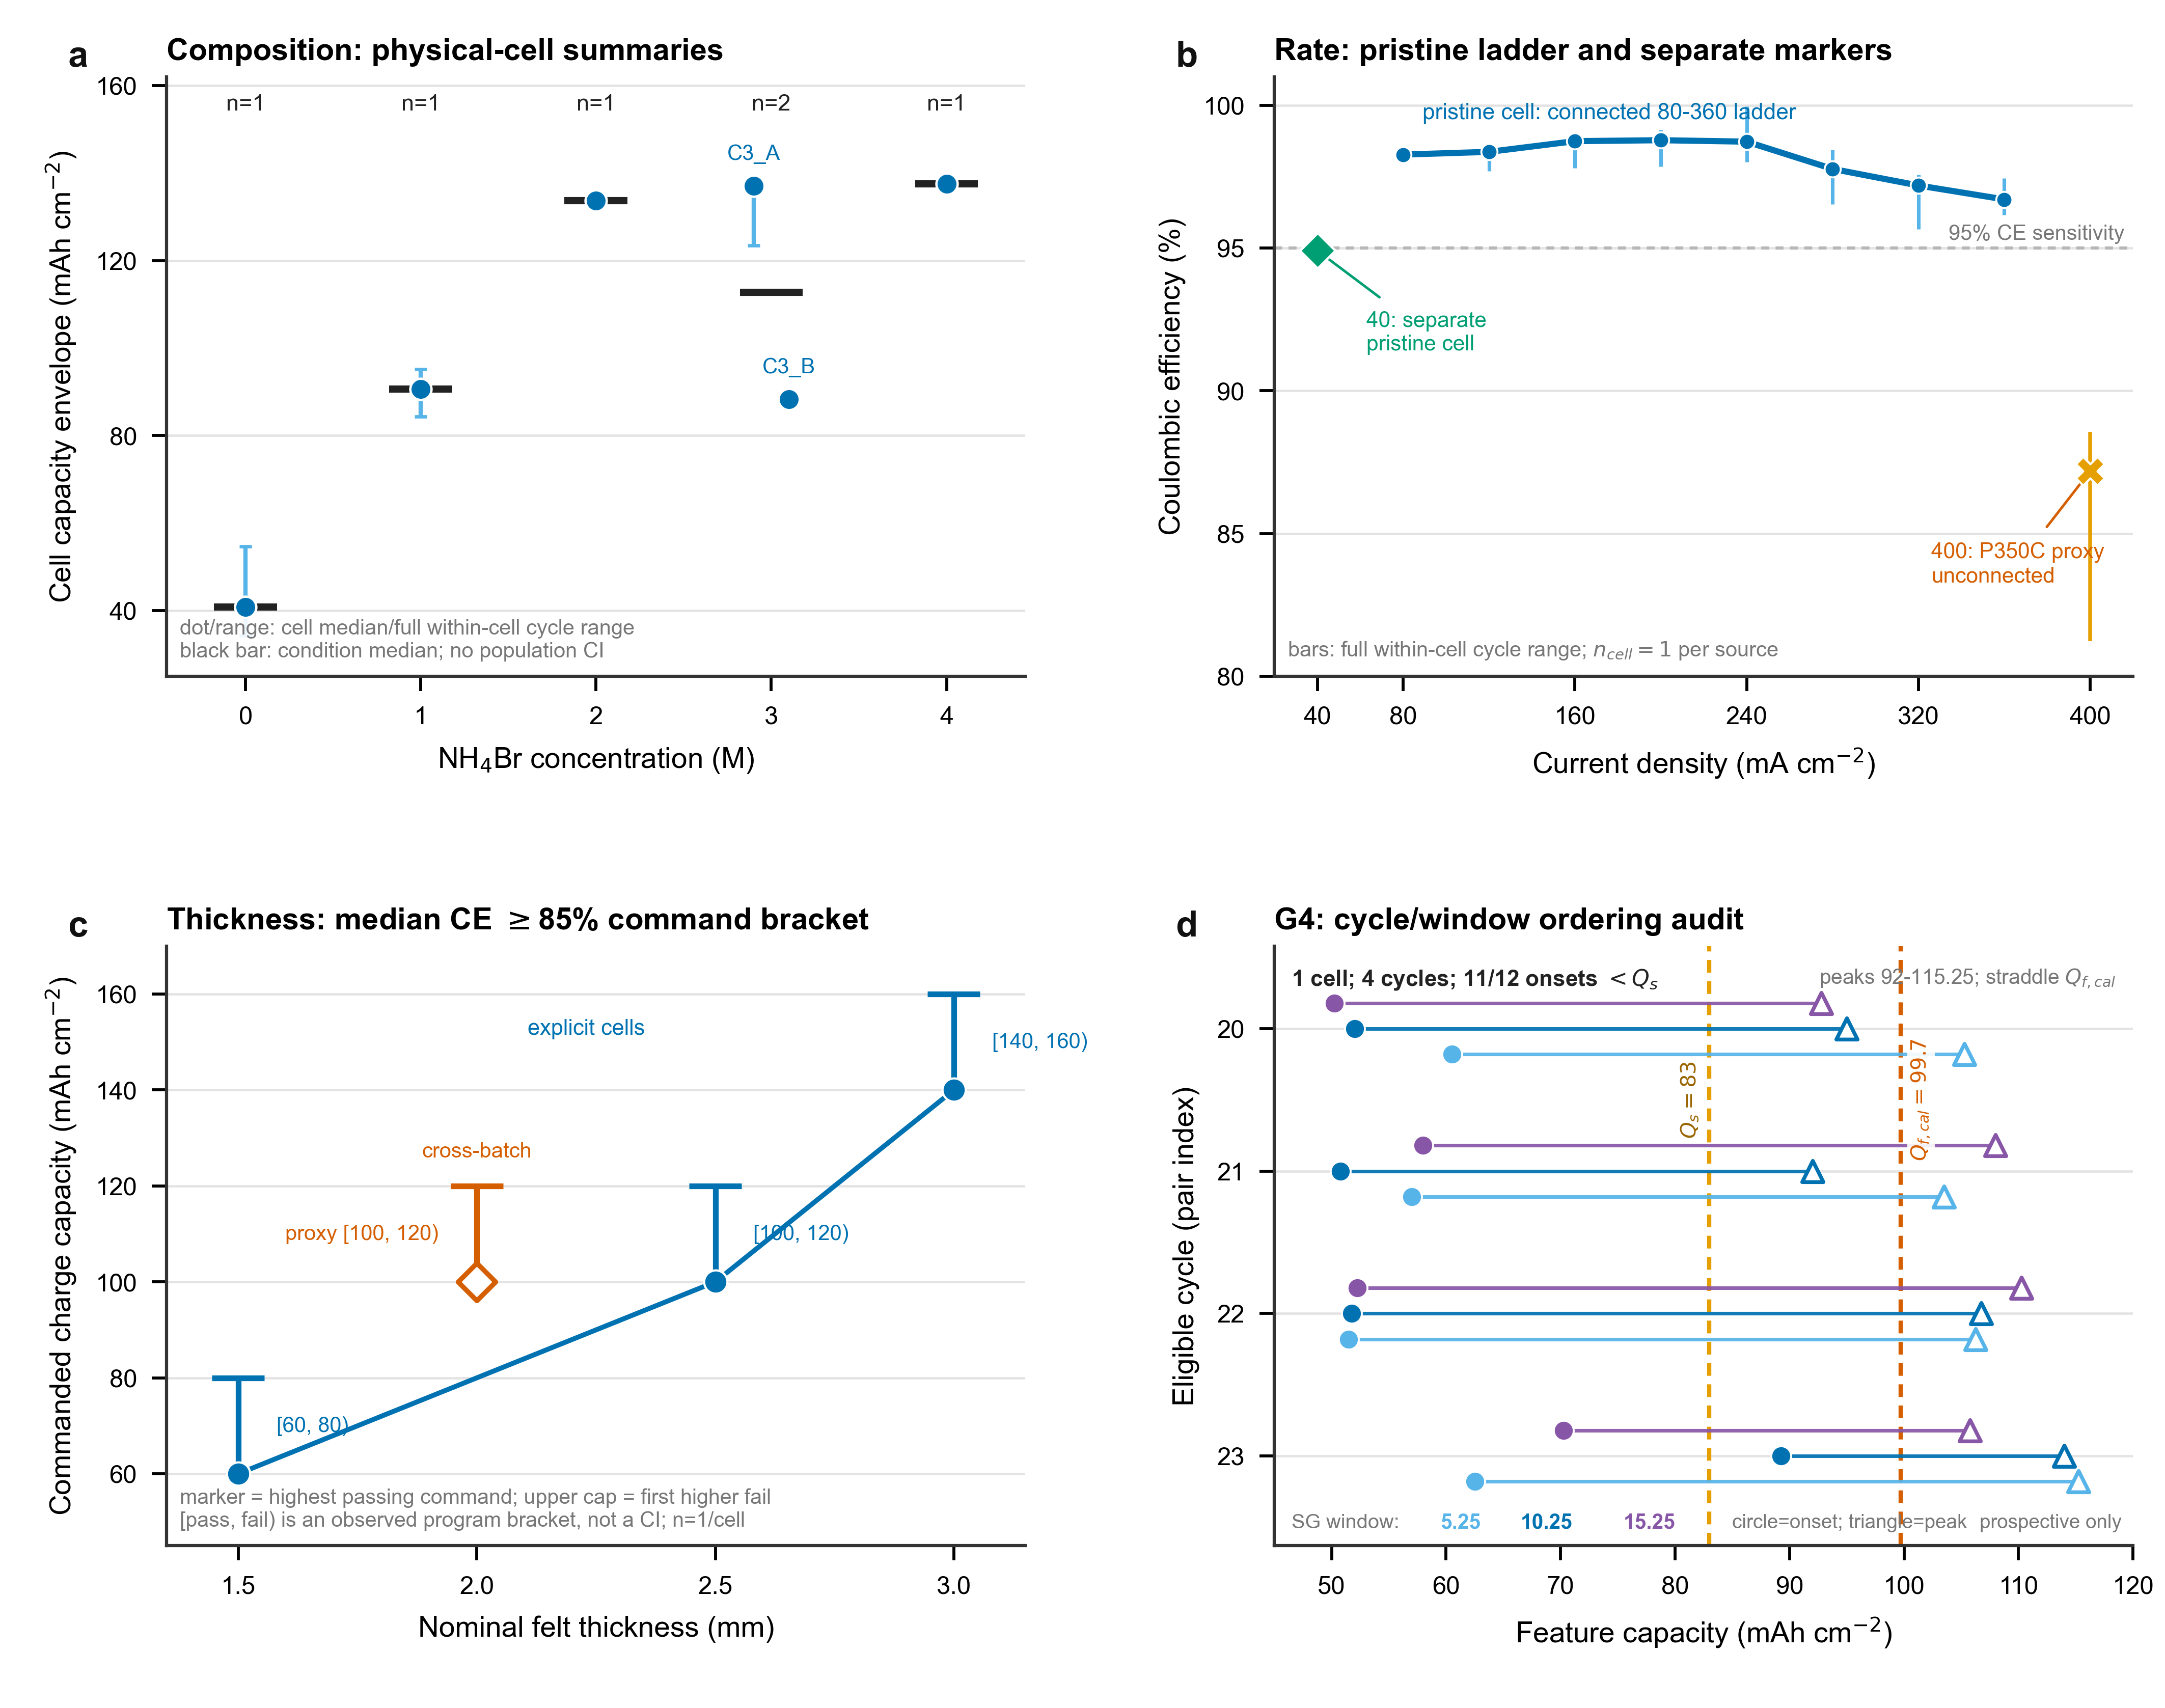
\includegraphics[width=\textwidth]{figures/Fig_R581_experimental_evidence.pdf}
\caption{\textbf{Existing full-cell evidence provides protocol-bounded stress tests rather than independent
validation of the modeled event ordering.} (a)~Cell-level delivered-capacity envelopes across the reconstructed
NH4Br composition series. Blue symbols are conservatively identified physical cells; vertical bars are full
within-cell cycle ranges at the selected command and black bars are condition medians. The independent-cell
counts are 1, 1, 1, 2 and 1 at 0--4~M. (b)~Coulombic efficiency across the 4~M rate evidence. Only the
80--\SI{360}{mA.cm^{-2}} same-cell pristine ladder is connected. The \SI{40}{mA.cm^{-2}} diamond is a separate
pristine cell and the \SI{400}{mA.cm^{-2}} cross is an unconnected P350C-positive/pristine-negative proxy.
The pristine ladder remains above the 95\% CE sensitivity level at its highest completed point and is
right-censored with respect to a pristine rate-failure current. (c)~Observed command brackets at the
prespecified within-cell median CE threshold of 85\%. Filled markers connect only the explicit 1.5, 2.5 and
3.0~mm cells; the open 2.0~mm marker is a cross-batch proxy. Each bracket is program resolution, not a
confidence interval. (d)~All four eligible G4 cycles from one cell under the primary 10.25 and prespecified
5.25/15.25~\si{mAh.cm^{-2}} derivative windows. Circles are rise onsets and open triangles are
$\mathrm{d}V/\mathrm{d}Q$ maxima. The model markers were not fitted to these traces: 11 of 12 onsets precede
$Q_{\mathrm s}$, whereas maxima straddle $Q_{\mathrm f,cal}$. Repeated cycles are within-cell observations;
no population confidence interval or inferential test is reported. Legacy acquisition names containing
``NH4Cl'' denote operator-confirmed NH4Br experiments under correction ID \texttt{EXP-META-001}.}
\label{fig:experimental-evidence}
\end{figure}

\section{Key parameters}
The cell/electrochemical inputs are listed in Table~\ref{tab:continuuminputs}; transport, speciation and
saturation inputs are listed separately in Table~\ref{tab:continuumtransport}.
\begin{table}[h]\centering\small
\caption{Central inputs of the registered continuum positive-electrode solve and the provenance of each value.
\emph{hardware/protocol} identifies an imposed scenario; \emph{literature reference/prior} identifies an
external scale that is not a measurement of the present concentrated electrolyte; \emph{lower-scale prior}
identifies an MD/mesoscale estimate; and \emph{empirical closure} or \emph{numerical regularizer} identifies a
modeling choice rather than an intrinsic property. The cell hardware (pristine graphite felt, Nafion and flow
frame) is that of our group's zinc-halide flow cells.}
\label{tab:continuuminputs}
\begin{tabular}{@{}p{0.25\textwidth}p{0.13\textwidth}p{0.30\textwidth}p{0.17\textwidth}@{}}
\toprule
quantity & symbol & value & provenance\\
\midrule
\multicolumn{4}{@{}l}{\textit{Cell and charge protocol}}\\
electrode area & $A$ & \SI{4}{cm^2} & prescribed\\
felt thickness; porosity rule & $L,\varepsilon(L)$ & \SI{2}{mm}; $1-0.30~\si{mm}/L$ & prescribed thickness; structural porosity closure\\
specific area & $a_s$ & $4\times10^{4}~\si{m^{-1}}$ & empirical geometry scale; no independent area measurement\\
membrane & --- & Nafion~212 ($\approx\!\SI{50}{\micro m}$) & prescribed\\
tank volume; flow rate & $V_{\mathrm{res}},Q$ & \SI{25}{mL}; \SI{50}{mL.min^{-1}} & prescribed\\
temperature & $T$ & \SI{293.15}{K} & prescribed model temperature\\
charge current density & $\iapp$ & \SI{400}{A.m^{-2}} ($\SI{40}{mA.cm^{-2}}$) & prescribed\\
electrolyte & --- & \SI{1}{M}~\ce{ZnI2}$+$\SI{4}{M}~\ce{NH4Br} & prescribed (representative)\\
\midrule
\multicolumn{4}{@{}l}{\textit{Positive (\ce{I2}/\ce{I^-}) electrochemistry}}\\
formal potential & $E^{0\prime}$ & \SI{0.548}{V} & prescribed model reference; no present-electrolyte anchor\\
exchange current density & $i_0$ & $5\times10^{4}~\si{A.m^{-2}}$ & fast-kinetics closure (not intrinsic)\\
transfer coefficients & $\alpha_a,\alpha_c$ & $1.0,\,1.0$ & symmetric Butler--Volmer closure\\
ionic conductivity & $\kappa_l$ & \SI{20}{S.m^{-1}} & undocumented prescribed value; no raw conductivity record located\\
Nernst-like total-pool reference & $c_{\mathrm{ref}}$ & $120~\si{mol.m^{-3}}$ & empirical reference concentration\\
native-solid exchange scale & $i_{0,\mathrm{dep}}^{\mathrm{base}}$ & $0.05~\si{A.m^{-2}}$ & empirical super-saturation-activated path\\
native-solid Tafel slope & $A_a$ & \SI{118}{mV} & prescribed path parameter\\
\bottomrule
\end{tabular}
\end{table}

\begin{table}[tbp]\centering\small
\caption{Transport, speciation and saturation inputs of the registered continuum solve. These values are
lower-scale or literature priors and model scenarios, not a fitted property set for the representative
supporting electrolyte.}
\label{tab:continuumtransport}
\begin{tabular}{@{}p{0.25\textwidth}p{0.13\textwidth}p{0.30\textwidth}p{0.17\textwidth}@{}}
\toprule
quantity & symbol & value & provenance\\
\midrule
free-\ce{I2} diffusivity & $D_{\ce{I2}}$ & $0.6\times10^{-9}~\si{m^2.s^{-1}}$ & lower-scale MD prior (Table~\ref{tab:mdprotocol})\\
\ce{I3^-},\,\ce{I2Br^-} diffusivity & --- & $0.5\times10^{-9}~\si{m^2.s^{-1}}$ & lower-scale MD prior; analogue force fields\\
mass-transfer length & $\delta$ & \SI{25}{\micro m} & sub-grid scenario parameter; not measured\\
deposit-free permeability & $\kappa_0$ & $1.0\times10^{-10}~\si{m^2}$ & prescribed felt-scale hydraulic value\\
electrolyte viscosity & $\mu$ & $2.2\times10^{-3}~\si{Pa.s}$ & prescribed hydraulic value; not measured in this project\\
electrolyte density & $\rho_l$ & \SI{1300}{kg.m^{-3}} & prescribed native-flow value\\
speciation constants & $K_{\mathrm I},K_{\mathrm{Br}}$ & $0.72,\,0.0115~\si{m^3.mol^{-1}}$ & conditional literature priors \citep{Palmer1984,Lee2023}\\
aqueous \ce{I2} solubility & $\csat$ & \SI{1.33}{mol.m^{-3}} & dilute-water reference \citep{Ramette1965}\\
salting-out factor & $\gamma_{\mathrm{salt}}$ & $3$ ($\csat^{\mathrm{eff}}\!\approx\!\SI{0.44}{mol.m^{-3}}$) & bounded cross-salt prior \citep{Palmer1984}\\
\ce{I2} molar volume & $V_m$ & $5.15\times10^{-5}~\si{m^3.mol^{-1}}$ & derived from $M_{\ce{I2}}/\rho_{\ce{I2}}$ in the model inventory\\
external areal dissolution fluxes & $k$ & $0.63,1.2$ (1 M); $2.2,5.1$ (2 M), $\times10^{-6}~\si{mol.cm^{-2}.s^{-1}}$ & condition/method specific \citep{Zhao2022}\\
\bottomrule
\end{tabular}
\end{table}
The authoritative deposited parameter-inventory CSV has SHA-256 prefix
\texttt{DDFA9B1B}; the complete digest is recorded in the release manifest.
Its internal description calls \SI{20}{S.m^{-1}} ``measured'', but the project contains no raw
electrolyte-conductivity record or documented geometry conversion that supports \SI{0.20}{S.cm^{-1}};
the available EIS files do not by themselves establish that bulk property. We therefore classify
$\kappa_l$ as an undocumented prescribed model value. The registered \SIrange{10}{40}{S.m^{-1}}
conductivity sweep changes the voltage channel but not the super-saturation marker, so this provenance gap
does not support a conductivity-identification claim. The exact $E^{0\prime}$, $i_0$, $c_{\mathrm{ref}}$,
$i_{0,\mathrm{dep}}^{\mathrm{base}}$, $A_a$, $a_s$ and $\delta$ likewise have no present-electrolyte
identification record and are kept explicitly as
model-reference, closure or scenario parameters. Absolute event capacities remain most sensitive to the
oxidized-carrier diffusivity and the $\gamma_{\mathrm{salt}}=2$--4 salting prior, as quantified below.
The reduced-model rate-closure efficiency $\phi_{\mathrm{ppt}}$ (relative sweeps $0.1$--$1$) is a
closure parameter calibrated on the production trajectory; it is not fixed by
$\epsislandhalf$ or $\epsfilmperc$. The native-solid and auxiliary-state constants are listed in
Table~\ref{tab:solidsource}.

\subsection{Native-solid path and auxiliary nucleation-state constants}\label{sec:solidsource}
The retained-solid inventory used by the continuum feedback is the COMSOL native deposited-species state,
\begin{equation*}
\partial_t\epss=V_m\frac{a_sj_{\mathrm{dep}}}{2F},\qquad
j_{\mathrm{dep}}=i_{0,\mathrm{dep}}^{\mathrm{base}}\max(S_{\mathrm{local}}-1,0)10^{\eta/A_a}.
\end{equation*}
The feature is active, uses the full pristine specific area $a_s$, and shares the implemented equilibrium
potential with the bare-carbon path. It converts only $0.552\%$ of the charge integrated over
$0$--$120~\si{mAh.cm^{-2}}$, but its contribution rises to $111.526~\si{A.m^{-2}}$ of the
$398.391~\si{A.m^{-2}}$ endpoint positive current. This late current partition produces
$\epss=3.21926\times10^{-3}$ and is therefore load-bearing.

A separate distributed ODE advances the auxiliary tracker $\varepsilon_{\mathrm{s,aux}}$ and the dimensionless
nucleation state $N_{\mathrm{I_2}}$:
\begin{align*}
\partial_t\varepsilon_{\mathrm{s,aux}}&=r_{\mathrm p}-r_{\mathrm d},\\
\partial_tN_{\mathrm{I_2}}&=\kappa_N(N_{\mathrm{target}}-N_{\mathrm{I_2}}),\\
r_{\mathrm p}&=\nu V_m a_s k_{\mathrm p}(\cf-\csat^{\mathrm{eff}})_{+}
\max\!\big(0,1-\epss/\varepsilon_0\big),\\
r_{\mathrm d}&=V_m a_s\theta_{\mathrm{case}} k_{\mathrm d}
(\csat^{\mathrm{eff}}-\cf)_{+}\frac{\epss}{\epss+\epss^{\mathrm{sm}}}.
\end{align*}
The registered target for the dimensionless nucleation state is
\begin{equation*}
N_{\mathrm{target}}=\min\!\left\{N_{\max},N_{\mathrm{ref}}\left[1+
\nu N_{\mathrm{sup}}(S_{\mathrm{local}}-1)_+^2
\left(e^{\min(|\eta_{\mathrm{cov}}|/\eta_{\mathrm{nuc}},8)}-1\right)\right]\right\},
\end{equation*}
with $N_{\mathrm{ref}}=1$, $N_{\mathrm{sup}}=500$, $N_{\max}=2\times10^7$,
$\eta_{\mathrm{nuc}}=\SI{3}{mV}$ and $\kappa_N=10^{-2}~\si{s^{-1}}$. This is a calibrated dynamic
accessibility-state construction, not a physical nucleation density.
Here $(\cdot)_+$ is a $\SI{0.02}{mol.m^{-3}}$-smoothed ramp and $\nu$ has a $0.03$ seed floor.
The auxiliary species source $(r_{\mathrm d}-r_{\mathrm p})/V_m$ enters the transported oxidized-pool
balance, while $N_{\mathrm{I_2}}$ enters the calibrated accessibility relation. The auxiliary solid tracker
ends at only $1.08328\times10^{-6}$, $2972$ times below the native deposited species, and is never reported as
the retained-solid inventory. The salting-out convention remains
$\csat^{\mathrm{eff}}=\csat/\gamma_{\mathrm{salt}}\approx\SI{0.44}{mol.m^{-3}}$. These constants are read
directly from the registered baseline \texttt{.mph}; this proves implementation identity, not experimental
provenance. The auxiliary $k_{\mathrm p}$ and $k_{\mathrm d}$ are empirical closures distinct from the
condition-specific literature areal dissolution fluxes used only as external kinetic scales.
\begin{table}[h]\centering\small
\caption{Native-solid and auxiliary-state values in the baseline solve, read from the deposited model copy and
classified by evidential role.}\label{tab:solidsource}
\begin{tabular}{@{}p{0.32\textwidth}p{0.16\textwidth}p{0.20\textwidth}p{0.24\textwidth}@{}}
\toprule
quantity & symbol & value & role\\
\midrule
native-solid exchange scale & $i_{0,\mathrm{dep}}^{\mathrm{base}}$ & $0.05~\si{A.m^{-2}}$ & empirical deposited-species path\\
native-solid Tafel slope & $A_a$ & \SI{118}{mV} & prescribed path parameter\\
auxiliary formation constant & $k_{\mathrm p}$ & $1\times10^{-9}~\si{m.s^{-1}}$ & empirical auxiliary rate closure\\
auxiliary dissolution constant & $k_{\mathrm d}$ & $5\times10^{-9}~\si{m.s^{-1}}$ & empirical auxiliary rate closure\\
nucleation relaxation rate & $\kappa_N$ & $10^{-2}~\si{s^{-1}}$ & calibrated dynamic-state closure\\
nucleation-target scales & $N_{\mathrm{ref}},N_{\mathrm{sup}},N_{\max}$ & $1,500,2\times10^7$ & calibrated dimensionless-state closure\\
nucleation overpotential scale & $\eta_{\mathrm{nuc}}$ & \SI{3}{mV} & calibrated dynamic-state closure\\
salting-out factor ($\csat^{\mathrm{eff}}=\csat/\gamma_{\mathrm{salt}}$) & $\gamma_{\mathrm{salt}}$ & $3$ & bounded cross-salt prior; not present-electrolyte data\\
super/under-saturation smoothing scale & --- & $0.02~\si{mol.m^{-3}}$ & numerical smoothing\\
nucleation seed floor & $\nu_0$ & $0.03$ & phenomenological initiation floor\\
Nernst-like total-pool reference & $c_{\mathrm{ref}}$ & $120~\si{mol.m^{-3}}$ & empirical reference concentration\\
solid-fraction regularizers & $\epss^{\mathrm{fl}},\epss^{\mathrm{sm}}$ & $10^{-9},\,10^{-8}$ & numerical regularizers\\
initial felt porosity & $\varepsilon_0$ & $0.85$ & prescribed structural scenario\\
\bottomrule
\end{tabular}
\end{table}
The solid molar volume is internally derived from the model inventory values
$M_{\ce{I2}}=\SI{253.80894}{g.mol^{-1}}$ and
$\rho_{\ce{I2}}=\SI{4.930}{g.cm^{-3}}$, giving \SI{51.48}{cm^3.mol^{-1}} and the implemented rounded
\SI{51.5}{cm^3.mol^{-1}}. It is a physical conversion, not a measurement performed in this project.
The production and physical accessibility expressions are defined separately in
Eqs.~\eqref{eq:closures-ref} and \eqref{eq:thetaisland}; neither physical threshold is substituted for the
production trajectory marker.

\section{Per-knob parameter-scan detail}\label{sec:si-knobs}
The main-text ranked sensitivity table condenses the native COMSOL parameter scans; the
per-family numbers behind each row are collected here. Each family is a \emph{separate} native scan with its
own fixed operating point (throughput $Q$, current density, thickness $L$, wetted area), so end-of-charge
voltages are not a shared baseline and are not comparable across families as absolute values; within a family
only the relative trend and the accessibility/solid-inventory outputs are used. Absolute voltage remains
conditional on the production accessibility calibration (Table~\ref{tab:bounds}, bound~i).

The tested fixed-$\csat$ scan families can be interpreted on a reduced-stress plane:
each knob is a distinct \emph{move} in the $(\Pi_{\mathrm{gen}},\Pi_{\mathrm{inv}})$ plane relative to one
saturation-marker boundary. With the intrinsic-$\csat$ definitions used here,
\begin{equation}
S_{\mathrm{base}}=\gamma_{\mathrm{salt}}
\frac{\Pi_{\mathrm{inv}}+\Pi_{\mathrm{gen}}}{\beta_{\mathrm{intra}}},
\qquad
S_{\mathrm{base}}=1\;\Longrightarrow\;
\Pi_{\mathrm{inv}}+\Pi_{\mathrm{gen}}=\frac{\beta_{\mathrm{intra}}}{\gamma_{\mathrm{salt}}}.
\label{eq:canonicalstress}
\end{equation}
Solving the same intrinsic-$\csat$ convention for the saturation-marker current gives
\begin{equation}
J_s^{+}(Q)=\frac{2F\Deff\csat}{\delta}
\left[\frac{\beta_{\mathrm{intra}}(Q)}{\gamma_{\mathrm{salt}}}
-\Pi_{\mathrm{inv}}(Q)\right]_{+}.
\label{eq:canonicaljs}
\end{equation}
Because the buffer at the marker is nearly constant across these scans
($\beta_{\mathrm{intra}}\approx760$) and $\gamma_{\mathrm{salt}}=3$, the marker is an almost fixed budget line
$\Pi_{\mathrm{gen}}+\Pi_{\mathrm{inv}}\approx253$. Rate, diffusivity and compression slide the point along
$\Pi_{\mathrm{gen}}$, state of charge climbs it in $\Pi_{\mathrm{inv}}$, salting-out shifts the whole plane,
and conductivity does not move it at all---the clean negative control. The solved flow rate also leaves the
point unmoved, but partly by construction: the fiber-scale boundary layer $\delta$ that carries the
mass-transfer stress is a sub-grid parameter decoupled from the electrode-scale Darcy field (main text,
operating-levers subsection), so the physical route by which higher flow thins $\delta$ and lowers
$\Pi_{\mathrm{gen}}$ is captured by the analytic $\delta/\Deff$ sweep, not by the flow scan.

\paragraph{Oxidized-carrier diffusivity (transport prior; effect $20.24$).} The oxidized-carrier diffusivity enters $S$
only through $\Pi_{\mathrm{gen}}\propto1/\Deff\propto1/D_0$, leaving $\Pi_{\mathrm{inv}}$ and $\beta$ untouched;
$\Pi_{\mathrm{gen}}$ is the diffusion-polarization overshoot needed to drive $i_{\mathrm{app}}/2F$ through the
Nernst layer $\delta$. Halving the diffusivity advances the marker $Q_{S\ge1}:83.1\to45.1$ (averaged peak
stress nearly unchanged, $S_{\mathrm{avg,peak}}=1.78$ vs.\ $1.76$ baseline---it is the marker shift, not the
averaged peak, that registers the doubled local overshoot), grows the solid inventory $52\times$
($\varepsilon_{s,\mathrm{end}}:3.22\times10^{-3}\to1.67\times10^{-1}$), saturates the production
accessibility-loss response
($\theta_{\mathrm{end}}\to1.000$, $A_{\mathrm{bare,end}}\approx2\times10^{-8}$), drops permeability
\SI{74}{\percent} ($K_{\mathrm{perm,end}}:0.956\to0.252$) and lifts the voltage
($V_{\mathrm{end}}:1.729\to\SI{1.849}{V}$). Doubling transport mirrors this through the same $1/D$ scaling
($S_{\mathrm{avg,peak}}:1.76\to1.22$, $Q_{S\ge1}=106.2$, $\varepsilon_{s,\mathrm{end}}=7.3\times10^{-5}$,
$A_{\mathrm{bare,end}}=0.666$); the end-state solid spans $\sim\!2290\times$ across the $\pm2\times$ bracket.
The marker response is mapped by a seven-point solved COMSOL sweep ($\Deff/D_0=0.5,0.6,0.8,1.0,1.2,1.5,2.0$,
giving $Q_{\mathrm s}=45.1,57.4,73.2,83.1,90.0,97.6,\SI{106.2}{\mAhcm}$; the diffusivity panel of the
main-text transport/formulation-envelope figure), so the continuous
$S(D)$ law is now resolved rather than inferred; because $\Deff$ folds in $\epsl^{1.5}$ a porosity change
would compound it, the diffusivity \emph{value} $D_0$ (an MD-bounded prior) remains the dominant source of
parametric uncertainty, so the load-bearing conclusion is the ranking, not a calibrated $D_0$.

\paragraph{Applied current density (rate; effect $4.10$).} Current density is the only operating variable that
enters $\Pi_{\mathrm{gen}}=i_{\mathrm{app}}\delta/(2FD_{\mathrm{eff}}\csat)$ directly and linearly. At fixed
\SI{40}{\mAhcm} throughput the peak stress rises $S_{\mathrm{avg,peak}}=0.328\to0.483\to0.924\to1.705$ at
$20,40,80,\SI{120}{mA.cm^{-2}}$ (a $5.2\times$ amplification for a $6\times$ rate increase); the system is
subcritical through \SI{80}{mA.cm^{-2}} and crosses $S=1$ between $80$ and \SI{120}{mA.cm^{-2}}. At the
crossing the solid jumps $\sim\!1900\times$ ($\varepsilon_{s,\mathrm{end}}:2.5\times10^{-7}\to4.8\times10^{-4}$),
accessible area collapses $0.999\to0.220$ ($\theta_{\mathrm{end}}=0.78$) and $V_{\mathrm{end}}=\SI{1.854}{V}$;
thresholds materialize only at \SI{120}{mA.cm^{-2}} ($Q_{S=1}=8.7$, $Q_{\theta=0.5}=31.3$). The buffer
co-depletes ($\beta_{\mathrm{end}}:1132\to565$, $2.0\times$), steepening failure beyond the linear
$\Pi_{\mathrm{gen}}$ term. This model saturation marker within a fixed-capacity sweep is distinct from the external,
condition- and method-specific dissolution-derived kinetic scales (approximately 122, 232, 425 and
\SI{984}{mA.cm^{-2}}) and must not be equated with them; the
high-rate branch (\SIrange{160}{320}{mA.cm^{-2}}) failed to converge, so the $S=1$ crossing is bracketed
rather than pinned.

\paragraph{Mechanical compression (effect $1.01$).} Compression acts through two opposing geometric channels
while leaving the chemistry untouched: thinning the felt ($L:3.0\to\SI{1.5}{mm}$) and lowering the porosity
($\epsl:0.900\to0.800$). The Bruggeman channel is weak and non-monotonic ($\Deff$ changes only
$\numrange{0.93}{1.11}\times$, $S_{\mathrm{avg,peak}}$ within $<\!2\%$). The decisive channel is the pore
volume $\epsl L$: at $Q=120$ the tight felt reaches $\theta_{\mathrm{cal,end}}=0.9998$ (surviving area
$2\times10^{-4}$) versus $0.920$ (surviving area $7.9\times10^{-2}$) for the loose felt---a $\sim\!400\times$
difference---so the production half-accessibility marker rises
$Q_{\langle\thetacal\rangle=0.5}:97.6\to\SI{103.3}{\mAhcm}$ ($+5.9\%$), while the saturation marker barely
moves ($Q_{S=1}:82.4\to84.3$). Because the calibrated relation reaches one half while $\epss$ is still
$\sim\!10^{-4}$, this result cannot be assigned the physical island or film-percolation threshold. The
experimental thickness series in Sec.~\ref{sec:compression} is a descriptive mixed-endpoint comparison, not
a validation of this model trajectory. The
non-monotonic $V_{\mathrm{end}}$ (\numrange{1.670}{1.776}{V}) is an ohmic/path-length artifact carrying no
failure information.

\paragraph{Active-material inventory (state of charge).} Charging raises $c_{\mathrm{I_2,tot}}$ so that
$\Pi_{\mathrm{inv}}\sim Q/Q_{\mathrm{base}}$ (a state-of-charge ramp on the baseline configuration, not an
independent molarity variation). The response is sharply super-linear:
$\varepsilon_{s,\mathrm{end}}=9.0\times10^{-8}$ at $Q=80$, $1.25\times10^{-4}$ at $100$, $3.22\times10^{-3}$ at
\SI{120}{\mAhcm}---a $25.8\times$ jump for a \SI{20}{\percent} inventory increase between $100$ and $120$, and
$3.6\times10^{4}\times$ across the window. The production trajectory localizes the averaged-saturation marker
$Q_{S=1}=83.1$ and
the calibrated marker $Q_{\mathrm f,cal}=99.59$, with $\langle\thetacal\rangle$ crossing $0.5$ near
\SI{100}{\mAhcm}
($\theta_{\mathrm{end}}:0.335\to0.519\to0.824$ over $Q=96\to100\to108$, saturating $0.990$ at $120$); the
accessibility collapse, not any conductivity change, drives $V_{\mathrm{end}}:1.427\to1.454\to1.601\to1.729$
over $Q=80\to100\to115\to120$. These voltage values are branch-specific outputs of the calibrated
accessibility relation.

\paragraph{Intrinsic and effective solubility (effect $9.55$).} The model keeps
$\csat=\SI{1.33}{\mol\per\meter\cubed}$ as a dilute-water intrinsic reference and represents the concentrated
electrolyte only through the bounded cross-salt factor
$\csat^{\mathrm{eff}}=\csat/\gamma_{\mathrm{salt}}$. A lower $\csat^{\mathrm{eff}}$ raises both inventory and
generation stresses and brings the registered $S=1$ marker forward---second-ranked overall behind the
diffusivity prior, registering at the solid-inventory node (weight $6.49$). The $\csat$ scan at fixed
$\gamma_{\mathrm{salt}}$ is therefore a reference-solubility uncertainty analysis, not a measurement of an
NH4Br-specific apparent solubility. Any additive that changes $\csat^{\mathrm{eff}}$ or $\beta$ requires its
own speciation/solubility data (Table~\ref{tab:bounds}, bound~iv).

\paragraph{Supporting bromide (within-cycle $\beta$ channel; effect $0.71$).} Within this fixed-electrolyte
scan, varying $c_{\mathrm{Br}}$ at fixed $\csat$ and $K_{\mathrm{Br}}$ perturbs neither numerator driver, so
the modeled local role is a speciation buffer,
$\partial S_{\mathrm{base}}/\partial c_{\mathrm{Br}}=-\gamma_{\mathrm{salt}}
(\Pi_{\mathrm{inv}}+\Pi_{\mathrm{gen}})K_{\mathrm{Br}}/\beta^2<0$.
In the native scan (\SI{2}{\Molar}, \SI{3}{\Molar}, \SI{5}{\Molar} at $\iapp=\SI{400}{A.m^{-2}}$,
$L=\SI{2.0}{mm}$, $Q=\SI{120}{\mAhcm}$) the buffer rises only modestly ($\beta_{\mathrm{end}}:543.2\to561.5$,
$+3.4\%$) and the stress response is weak ($S_{\mathrm{avg,peak}}:1.772\to1.743$, $Q_{S=1}:81.2\to84.0$,
$Q_{\langle\thetacal\rangle=0.5}:97.6\to100.7$). The one appreciable signature is the native deposited inventory
($\varepsilon_{s,\mathrm{end}}:7.47\times10^{-3}\to1.90\times10^{-3}$, $\sim\!3.9\times$; $A_{\mathrm{bare,end}}:
5.0\times10^{-3}\to1.5\times10^{-2}$). A within-cycle buffer already near $\beta\approx550$ has almost no
marginal leverage. The descriptive cross-composition series in Sec.~\ref{sec:chemfit} does not identify a
transferable accommodation factor. NH4Br remains the representative supporting electrolyte, not the subject
of the positive-electrode mechanism.

\paragraph{Electrode specific (wetted) area (effect $0.54$, unresolved).} Under the global galvanostatic
areal balance, $a_sL$ cancels from $\Pi_{\mathrm{gen}}$; changing $a_s$ can instead redistribute local current
and reaction area. Only the low-area branch converged. That single point ($a_s\!\times\!0.5$) shifts
$S_{\mathrm{avg,peak}}$ by $+2.4\%$ but ends with less calibrated blocking, so neither the sign nor a global
$1/a_s$ law is identified.

\paragraph{Non-drivers: conductivity (clean) and flow (partly by construction; effect $0.12$--$0.84$).}
Liquid conductivity $\sigma_l$
(\SIrange{10}{40}{\siemens\per\meter}) and electronic conductivity $\sigma_s$
(\SIrange{80}{320}{\siemens\per\meter}) enter only the charge-transport law, never
$S$---the clean negative control. Flow $Q_{\mathrm{flow}}$ enters the electrode-scale advection but not the
fiber-scale boundary layer $\delta$, which is a sub-grid parameter; its pinned saturation marker is therefore partly a
model-construction result (the physical flow$\to\delta\to\Pi_{\mathrm{gen}}$ route is carried by the analytic
$\delta/\Deff$ sweep). They swing $V_{\mathrm{end}}$ by $77$ and \SI{141}{mV} (the largest ohmic excursions in
the study) yet leave the saturation marker pinned at $Q_{S\ge1}=83.1$ ($Q_{\mathrm{flow}}$ moves it by $0.22$). The one nuance is $\sigma_s$:
a poorly conducting felt crowds the reaction toward the membrane side and raises the local \ce{I2} flux
(end-state $\epss$ up $\sim\!4.5\times$), but this is post-marker current crowding, not a shift of the
supersaturation threshold.

\section{Transport-channel accounting}\label{sec:channelsi}
\begin{table}[h]\centering\small
\caption{\textbf{Transport-channel accounting.} Which transport channels the positive-electrode model
carries, their governing variables and effect, and what a new electrolyte would require. The accessibility
and diffusive mass-transfer channels are both \emph{in} the model; the smooth geometric permeability is
resolved; viscosity enters only as a hydraulic multiplier; discrete/local blockage is explicitly out of
scope.}
\label{tab:channels}
\begin{tabular}{p{0.16\textwidth}p{0.15\textwidth}p{0.12\textwidth}p{0.24\textwidth}p{0.19\textwidth}}
\toprule
channel & variable(s) & in the model? & main effect & new data to extrapolate \\
\midrule
accessibility (active area) & $\thetacal$, $\thetaisland$ & production calibrated; physical alternative matched & $(1-\theta)$ prefactor on reaction kinetics and charge voltage & deposit imaging / morphology-resolved accessibility \\
diffusive mass transfer & $\Deff$, $\delta$ & yes (in $\Pi_{\mathrm{gen}}$) & sets $S_{\mathrm{base}}$ and the saturation marker via $\Pi_{\mathrm{gen}}\propto1/\Deff$ & $D(c)$, boundary layer $\delta$ \\
hydraulic & $K(\epss)$, $\mu$ & $K$ yes (geometric); $\mu$ as a multiplier & Darcy pressure $\Delta p\propto\mu/K$ & $\mu(c)$ \\
chemistry / accommodation & $\beta_{\mathrm{intra}}$, $\Lambda^{\mathrm{rel}}_{X}$, $\csat$ & buffer solved; $\Lambda^{\mathrm{rel}}_{X}$ empirical and not transferable & free-\ce{I2} activity / accommodation, shifting the modeled saturation marker & speciation / solubility of the new ligand \\
discrete / local blockage & local pore-throat clog, collector-side shell & no (smooth closures only) & late or local hydraulic / shell failure & tomography / imaging \\
\bottomrule
\end{tabular}
\end{table}

\section{Negative-electrode scenario estimate}\label{sec:cdrsi}
Figure~\ref{fig:cdr} reports an illustrative current-density-ratio calculation to expose the consequence of
declared zinc concentration, diffusivity and boundary-layer assumptions. It is not used to assert the actual
negative-electrode margin.

\begin{figure}[h]\centering
\includegraphics[width=0.52\linewidth]{figures/Fig_R563_cdr_minicalc.pdf}
\caption{\textbf{Negative-electrode current-density-ratio (CDR) regime sanity check.} The ratio
$\mathrm{CDR}=j/j_{\mathrm{lim}}$ measures how close the applied current density $J$ sits to an illustrative
zinc diffusion limit $j_{\mathrm{lim}}=nFD_{\ce{Zn}}c_{\ce{Zn}}/\delta$. The calculation uses $n=2$ and
$D_{\ce{Zn}}\!\sim\!7\times10^{-10}~\si{\meter\squared\per\second}$ from the cited transport context
\citep{ZnBr_CurrentDist2024}; $c_{\ce{Zn}}=\SI{1}{\mol\per\liter}$ and
$\delta=\SI{25}{\micro\meter}$ are declared scenario assumptions, giving
$j_{\mathrm{lim}}\!\approx\!\SI{540}{mA.cm^{-2}}$. Across the tested moderate-current window
($40$--$\SI{100}{mA.cm^{-2}}$, shaded) the scenario ratio stays $\mathrm{CDR}\lesssim0.2$ (points at $0.07$
and $0.19$); at $J=\SI{300}{mA.cm^{-2}}$ it is $0.56$, and by definition it reaches unity at the assumed
$j_{\mathrm{lim}}$ (dashed line). The dashed line is an illustrative diffusion limit, not a dendrite-onset
criterion. This is a \emph{regime sanity
check, not a solved negative-electrode model}: it shows the consequence of the stated $c_{\ce{Zn}}$ and
$\delta$ assumptions; it does not establish the actual negative-electrode mass-transfer margin or resolve dendrite morphology, interfacial
kinetics, or the full negative-electrode transport problem.}
\label{fig:cdr}
\end{figure}

\section{Limitations and scope}\label{sec:limits}
The continuum model is a calibrated mechanism scaffold, not an exact voltage validator or an inverse
morphology measurement. The matched comparison establishes that one accessibility-expression change,
under otherwise fixed continuum settings, changes the endpoint voltage by $-\SI{288.156}{mV}$ and changes
the solid-inventory trajectory. It does not establish which closure represents the real deposit. The DFT and
MD calculations supply placement tendencies and bulk-carrier bounds; the fibre and pore calculations are
geometric closure tests, not imaged electrode microstructures. The experimental composition, compression and
rate datasets contain one physical cell per condition/source except for two cells at 3 M NH4Br; they are
descriptive and protocol-bounded. The full-cell derivative reconstruction is likewise one cell and does not
validate the modeled event ordering. Failure-regime impedance spectra were non-interpretable and are excluded
from the mechanism claim.

The scope is deliberately positive-electrode and branch-specific. The model resolves the
$\ce{I^-}/\ce{I2}$ positive branch under a representative NH4Br supporting electrolyte. Published
dissolution measurements supply external, condition-specific kinetic scales rather than a validated ceiling
for this electrolyte. Negative zinc morphology and membrane damage \citep{Richtr2026,Guo2025}, dissolved
polyiodide shuttle \citep{Wei2025}, and high-bromide four-electron interhalogen chemistry
\citep{Liao2025,HuangIL2025,ChenComplex2026} are not solved; they remain literature-anchored external regimes.
NH4Br and bromide are supporting conditions, not the scientific protagonist.

\begin{table}[h]\centering\small
\caption{\textbf{Scope and bounds of the positive-electrode analysis.} Each modeling choice and its
consequence for the corresponding claim.}
\label{tab:bounds}
\begin{tabular}{p{0.13\textwidth}p{0.40\textwidth}p{0.37\textwidth}}
\toprule
bound & statement & consequence for claims \\
\midrule
(i) voltage &
the production voltage is conditional on the calibrated accessibility relation; the matched physical case is
$288.156$ mV lower at the endpoint &
the difference quantifies model-closure sensitivity, not real morphology or absolute-voltage validation \\
(ii) closure &
the true-mesh production control reaches $Q_{\mathrm f,cal}=99.4637$; the coupled physical-dense case does not reach
$\langle\theta\rangle=0.5$ by $Q=120$ &
$Q_{\mathrm f,cal}$ and $\Delta Q_{\mathrm{cal}}$ are production-closure outputs; no cross-closure invariance is claimed \\
(iii) thresholds &
$\epscalstar$, $\epsislandhalf$ and $\epsfilmperc$ have different definitions &
none is substituted for another or reported as an experimental material constant \\
(iv) constants &
$\csat=\SI{1.33}{\mol\per\meter\cubed}$ is fixed \citep{Ramette1965} (above the $1.1$--$\SI{1.2}{mM}$
reported elsewhere \citep{Bentley2015,Lee2023}) and sets $S=1$ linearly; the reduced solid-formation efficiency
$\phi_{\mathrm{ppt}}$ is calibrated to the production trajectory, not measured and not the native-path current &
$\csat$, $\gamma_{\mathrm{salt}}$, $D_{\mathrm{eff}}$ and the closure dominate absolute marker positions \\
(v) supporting electrolyte &
$\beta_{\mathrm{intra}}$ is reconstructed algebraically within the representative electrolyte; cross-composition accommodation is
empirical and not transferable &
the reconstructed NH4Br series supports only a descriptive condition trend; bromide is not the central mechanism \\
(vi) experiments &
compression has $n_{\mathrm{cell}}=1$ per thickness, composition has $1/1/1/2/1$ cells, each rate source has
$n_{\mathrm{cell}}=1$, and G4 has one cell &
no population inference, quantitative threshold validation or cycle-as-cell resampling is claimed \\
(vii) failure mode &
the pore network tests smooth bulk permeability only; discrete local blockage, deep hydraulic runaway and
mechanical failure are not resolved &
out of scope; no unique connected-film or pore-blockage morphology is claimed \\
\bottomrule
\end{tabular}
\end{table}


\begin{figure}[tbp]\centering
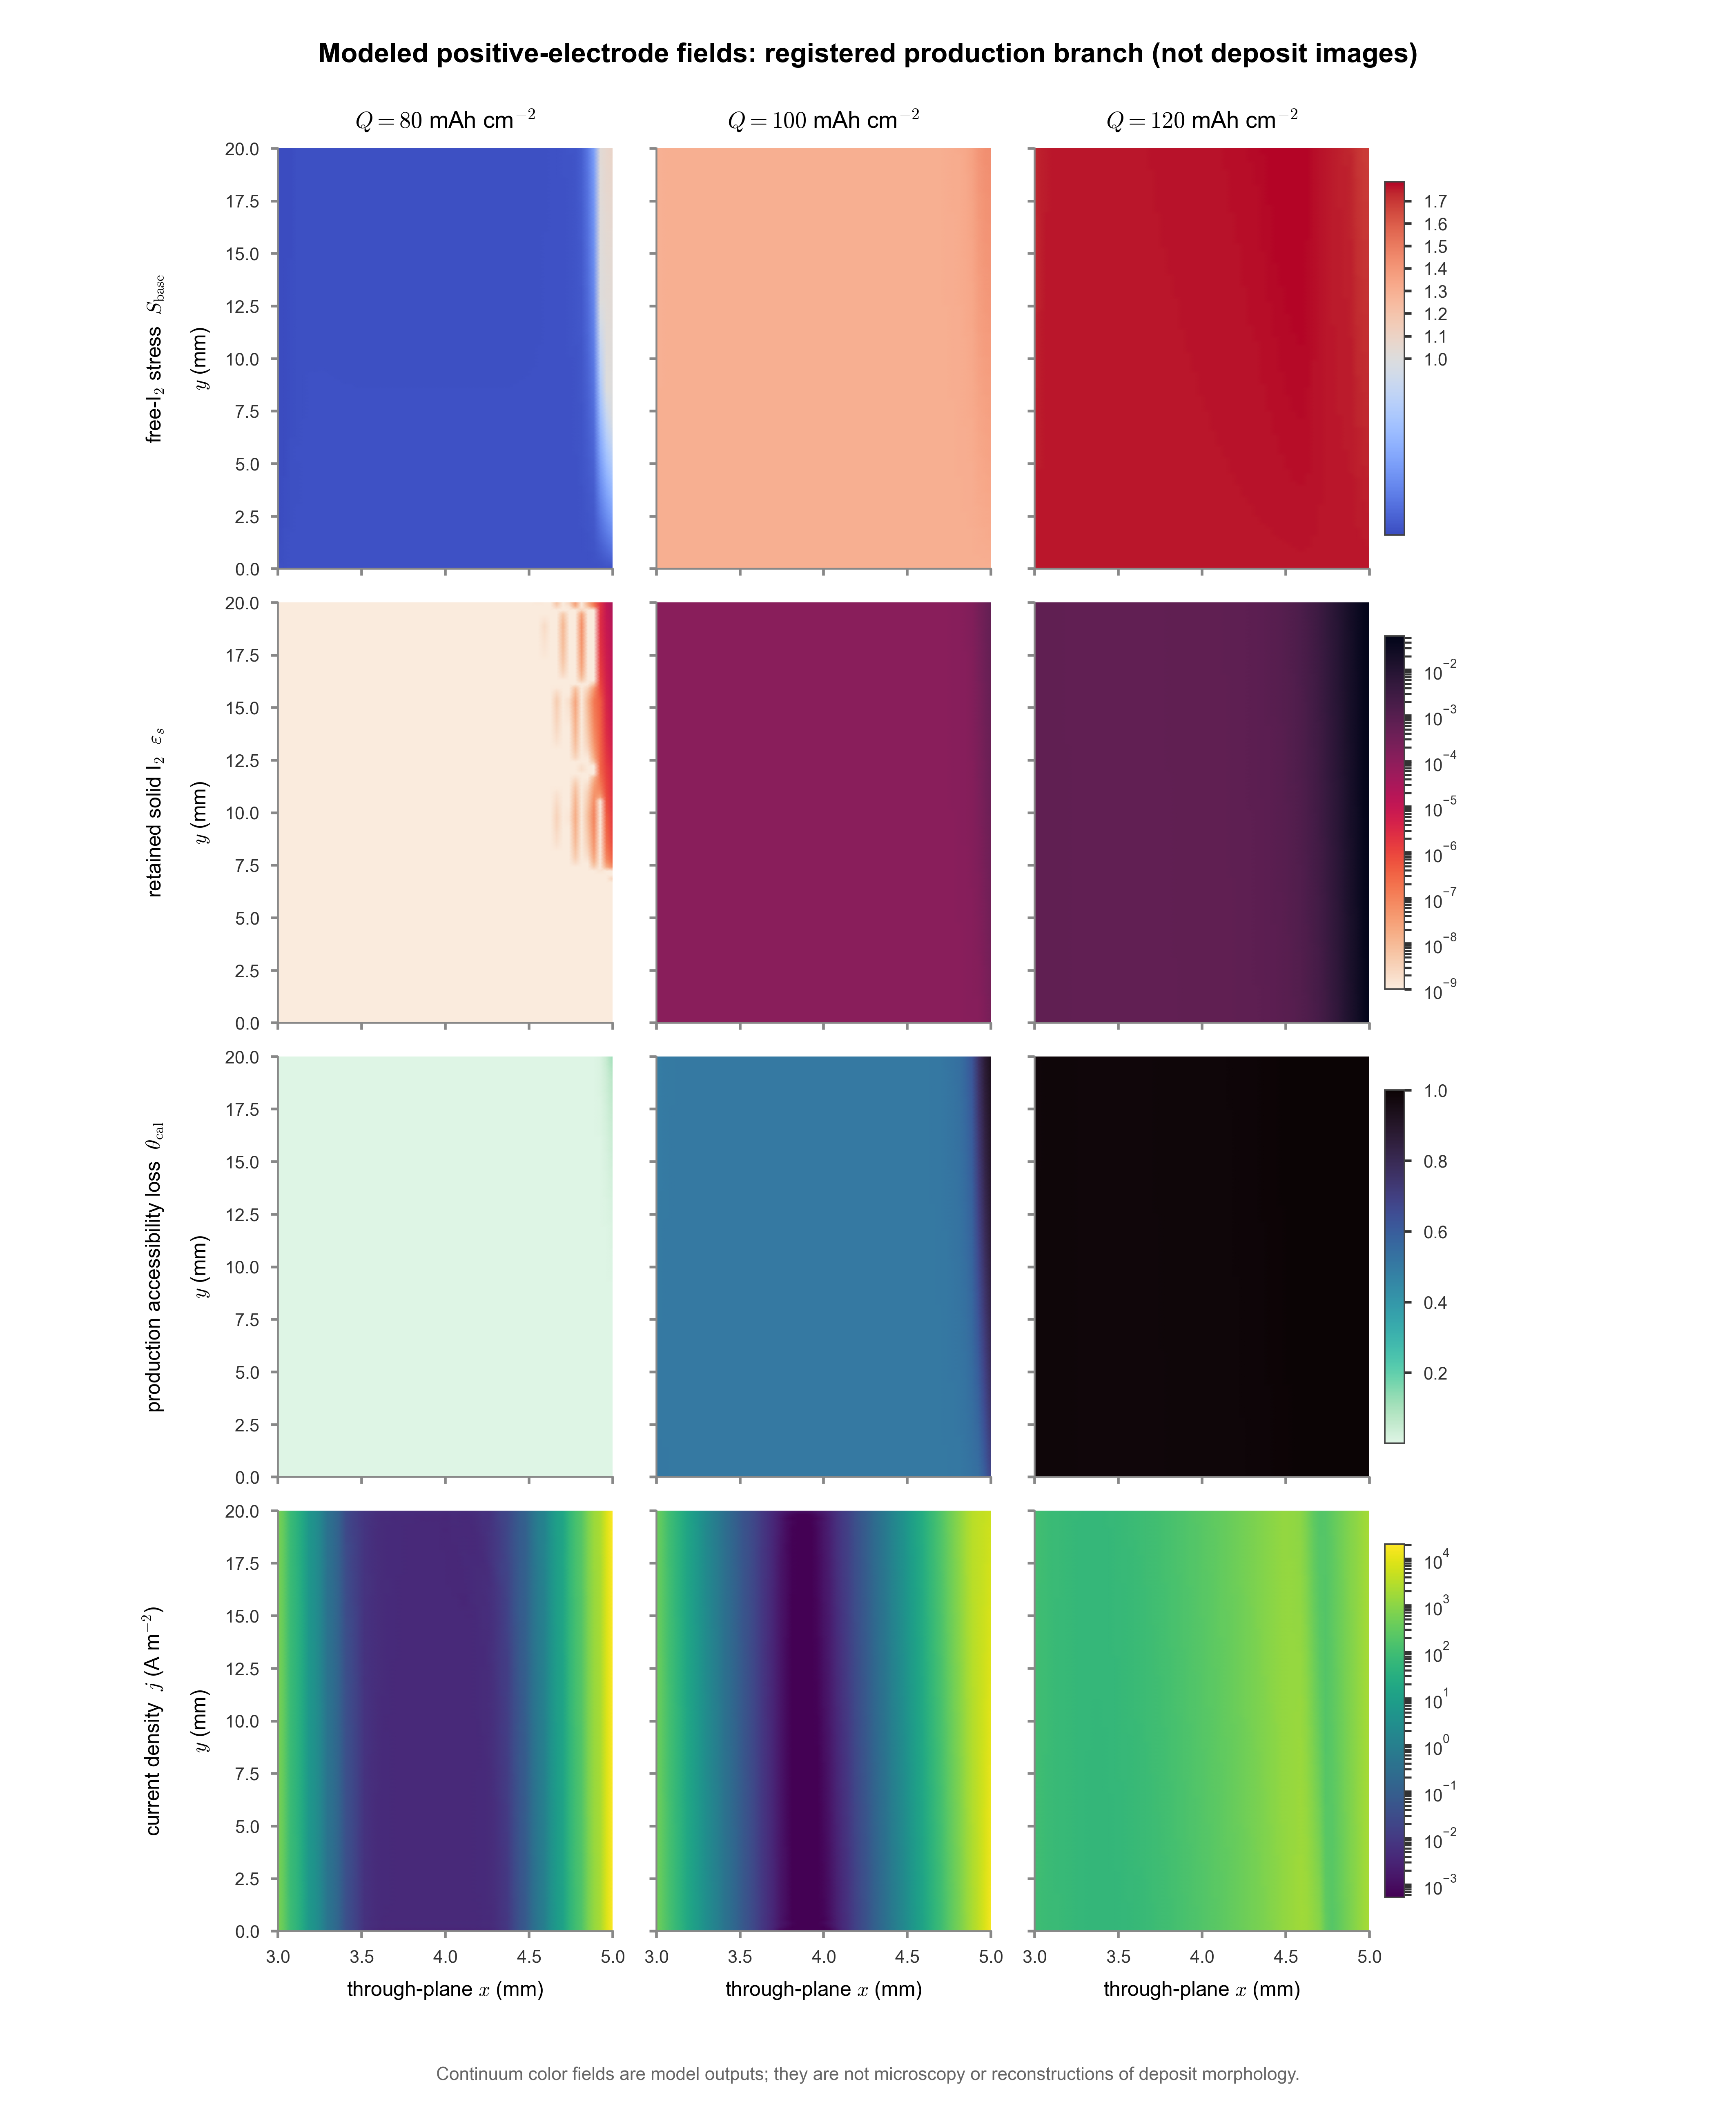
\includegraphics[width=0.86\textwidth]{figures/Fig_R545_spatial_maps.pdf}
\caption{\textbf{Two-dimensional production-model field maps of the positive electrode} over the domain of
Fig.~\ref{fig:geometry} (through-plane $x$ horizontal, collector at $3$\,mm to separator at $5$\,mm; flow
direction $y$ vertical), at three capacities $Q=80/100/120~\mAhcm$. Rows (top to bottom): free-\ce{I2}
super-saturation $S_{\mathrm{base}}$, retained solid $\epss$, calibrated accessibility loss $\thetacal$, and
total current density $j$. \emph{What to notice}:
retained solid is concentrated near the separator face, total current remains spatially nonuniform, and $S$
stays a smooth through-plane gradient. These are fields of the registered calibrated production branch, not
images of the real deposit.}
\label{fig:spatial}
\end{figure}

\begin{figure}[tbp]\centering
\includegraphics[width=0.86\textwidth]{figures/Fig_R556_mesoscale_renders.pdf}
\caption{\textbf{Physical mesoscale model geometries.} (a) The isolated-island single-fibre deposition cell
($r_f=\SI{7.5}{\micro m}$, $\epsl=0.85$) with stochastically nucleated \ce{I2} islands, and (b) the
pore-throat network after deposit. The render depicts the assumed physical-island and network geometries; it
is not a reconstruction of the production effective morphology and does not establish the presence or
absence of a continuous or pore-spanning deposit in the experiment.}
\label{fig:mesomodel}
\end{figure}

\clearpage
\bibliographystyle{unsrtnat}
\bibliography{refs}

\end{document}
